%%%%%%%%%%%%%%%%%%%%%%%%%%%%%%%%%%%%%%%%%
% Beamer Presentation
% LaTeX Template
% Version 1.0 (10/11/12)
%
% This template has been downloaded from:
% http://www.LaTeXTemplates.com
%
% License:
% CC BY-NC-SA 3.0 (http://creativecommons.org/licenses/by-nc-sa/3.0/)
%
%%%%%%%%%%%%%%%%%%%%%%%%%%%%%%%%%%%%%%%%%

%----------------------------------------------------------------------------------------
%	PACKAGES AND THEMES
%----------------------------------------------------------------------------------------
\PassOptionsToPackage{dvipsnames}{xcolor}

\documentclass[xcolor=dvipsnames]{beamer}

\mode<presentation> {

% The Beamer class comes with a number of default slide themes
% which change the colors and layouts of slides. Below this is a list
% of all the themes, uncomment each in turn to see what they look like.

%\usetheme{default}
%\usetheme{AnnArbor}
%\usetheme{Antibes}
%\usetheme{Bergen}
%\usetheme{Berkeley}
%\usetheme{Berlin}
%\usetheme{Boadilla}
%\usetheme{CambridgeUS}
%\usetheme{Copenhagen}
%\usetheme{Darmstadt}
%\usetheme{Dresden}
%\usetheme{Frankfurt}
%\usetheme{Goettingen}
%\usetheme{Hannover}
%\usetheme{Ilmenau}
%\usetheme{JuanLesPins}
%\usetheme{Luebeck}
\usetheme{Madrid}
%\usetheme{Malmoe}
%\usetheme{Marburg}
%\usetheme{Montpellier}
%\usetheme{PaloAlto}
%\usetheme{Pittsburgh}
%\usetheme{Rochester}
%\usetheme{Singapore}
%\usetheme{Szeged}
%\usetheme{Warsaw}

% As well as themes, the Beamer class has a number of color themes
% for any slide theme. Uncomment each of these in turn to see how it
% changes the colors of your current slide theme.

%\usecolortheme{albatross}
%\usecolortheme{beaver}
%\usecolortheme{beetle}
%\usecolortheme{crane}
\usecolortheme{dolphin}
%\usecolortheme{dove}
%\usecolortheme{fly}
%\usecolortheme{lily}
%\usecolortheme{orchid}
%\usecolortheme{rose}
%\usecolortheme{seagull}
%\usecolortheme{seahorse}
%\usecolortheme{whale}
%\usecolortheme{wolverine}

%\setbeamertemplate{footline} % To remove the footer line in all slides uncomment this line
%\setbeamertemplate{footline}[page number] % To replace the footer line in all slides with a simple slide count uncomment this line

\setbeamertemplate{navigation symbols}{} % To remove the navigation symbols from the bottom of all slides uncomment this line
}



\input inputs/packages.tex
\input inputs/abbreviations.tex
\input inputs/commands.tex

%----------------------------------------------------------------------------------------
%	TITLE PAGE
%----------------------------------------------------------------------------------------

\newcommand\meeting{PhD thesis defense}

\title[\meeting]{Measurement of the photon energy spectrum in
inclusive radiative \texorpdfstring{$B$}{B} meson decays using the
hadronic-tagging method} % The short title appears at the bottom of every slide, the full title is only on the title page

\author[Henrikas Svidras]{\texorpdfstring{\footnotesize \underline{Henrikas Svidras}}{Henrikas Svidras}} % Your name
%\subject{\text{\small KEK, Tsukuba}}
\institute[DESY] % Your institution as it will appear on the bottom of every slide, may be shorthand to save space
{
\text{\large \meeting}
\vspace{-10pt}
}
\titlegraphic{
\includegraphics[width=1.8cm]{logos/uni_profile_93570.jpg}
\includegraphics[width=2cm]{logos/DESY.png}\hspace*{4.75cm}~%
   
\includegraphics[width=2cm]{logos/belle2.png}
}

\date{March 13, 2023} % Date, can be changed to a custom date

\begin{document}

\setbeamercolor{background canvas}{bg=}
{\setbeamertemplate{footline}{} 
\begin{frame}
\titlepage % Print the title page as the first slide
\end{frame}
}
\addtocounter{framenumber}{-1}


%----------------------------------------------------------------------------------------
%	INTRO
%----------------------------------------------------------------------------------------
\section{Introduction}

\begin{frame}

   \centering

{\LARGE Measurement of the photon energy spectrum in
{\color{OrangeRed}inclusive} {\color{YellowGreen}radiative} \texorpdfstring{$B$}{B} meson decays using the
{\color{MidnightBlue}hadronic-tagging} method}

\vspace{10pt}

\textbf{Let's look at these three terms closer}

\end{frame}

\begin{frame}{Introduction: radiative \safeB meson decays}
\centering\scriptsize
{\normalsize What are \textbf{radiative $\bm{B}$} decays?
\begin{columns}
   \column{0.4\textwidth}
   \begin{tikzpicture}
    \begin{feynman}
    \vertex (i1){b};
    \vertex[right =1.2cm of i1] (a);
    \vertex[right=0.85cm of a] (b);
    \vertex[right=0.85cm of b] (c);
    \vertex[right=1.2cm of c] (o1) {s,d};
    \vertex[below=2em of c] (g1);
    \vertex[right=2em of g1] (o2) {$\gamma$};
    
    \diagram* {
    (i1) -- [fermion] (a) -- [fermion, edge label =\(uct\)] (c) -- [fermion] (o1),
    (a) -- [boson,half left, edge label = \(W^{\pm}\)] (c),
    (b) -- [photon] (o2),
    };
    \end{feynman}
\end{tikzpicture}
    
   \column{0.4\textwidth}
   \begin{tikzpicture}
    \begin{feynman}
    \vertex (i1){b};
    \vertex[right =1.2cm of i1] (a) ;
    \vertex[right=0.85cm of a] (b);
    \vertex[right=0.85cm of b] (c);
    \vertex[right=1.2cm of c] (o1) {s,d};
    \vertex[below=2em of c] (g1);
    \vertex[right=2em of g1] (o2) {$\gamma$};
    
    \diagram* {
    (i1) -- [fermion] (a) -- [boson, edge label =\(W^{\pm}\)] (c) -- [fermion] (o1),
    (a) -- [fermion,half left, edge label = \(uct\)] (c),
    (b) -- [photon] (o2),
    };
    \end{feynman}
\end{tikzpicture}
    
\end{columns}
}

\begin{itemize}
   \item Rare decays: \textbf{forbidden at tree level} in the Standard Model!
   \item \textbf{New particles} can appear \textbf{in the loops}, one of many examples:
\end{itemize}
{\normalsize
\begin{columns}
   \column{0.4\textwidth}
   \begin{tikzpicture}
    \begin{feynman}
    \vertex (i1){b};
    \vertex[right =1.2cm of i1] (a) ;
    \vertex[right=0.85cm of a] (b);
    \vertex[right=0.85cm of b] (c);
    \vertex[right=1.2cm of c] (o1) {s,d};
    \vertex[below=2em of c] (g1);
    \vertex[right=2em of g1] (o2) {$\gamma$};
    
    \diagram* {
    (i1) -- [fermion] (a) -- [scalar, edge label =\(H^{\pm}\)] (c) -- [fermion] (o1),
    (a) -- [fermion,half left, edge label = \(uct\)] (c),
    (b) -- [photon] (o2),
    };
    \end{feynman}
\end{tikzpicture}
\end{columns}
}
\begin{itemize}
   \item In the case of \btosgamma: $\mathcal{B}\sim10^{-4}$.
   \item[\ra] Accessible with smaller datasets than e.g. $b\to s\ell\ell$, where $\mathcal{B}\sim10^{-6}$
\end{itemize}

\end{frame}

% \begin{frame}{Introduction: inclusive \safeB meson decays}
%    \centering\scriptsize
%    {\normalsize What are \textbf{inclusive $\bm{B}$} decays?}

%    \vspace{10pt}

%    \begin{itemize}
%       \item $B$ mesons are the \textbf{lightest mesons involving a $\bm{b}$ quark}
%       \item[\ra] decays always involve one or more flavour/generation changes!
%       \item[\ra] plethora of final decay states from $u, d, c, s$ quarks
%    \end{itemize}

%    \vspace{10pt}

%    \begin{columns}
%       \column{0.5\textwidth}
%       \centering
%          \textbf{Exclusive}: pick a particular state and study its properties
%             \begin{itemize}
%                \item $B^0\to{K^0}^*(892)\gamma$
%                \item $B^+\to K^+\mu^+\mu^-$
%             \end{itemize}
%       \column{0.5\textwidth}
%       \centering
%          \textbf{Inclusive}: study all states originating from the associated quark
%          \begin{itemize}
%             \item $B\to X_s \gamma$
%             \item $B\to X_u \ell \nu$
%          \end{itemize}
%    \end{columns}
   
%    \vspace{10pt}
%    Just a couple from many of potential examples!

% \end{frame}

\begin{frame}{Introduction: inclusive \safeB meson decays}
   \centering\scriptsize
   
   \vspace{5pt}
   
   {\normalsize What are \textbf{inclusive $\bm{B}$} decays?}
   
   \vspace{5pt}

   \begin{columns}
      \column{0.33\textwidth}
      \pgfdeclarelayer{bg}    % declare background layer
\pgfsetlayers{bg,main}  % set the order of the layers (main is the standard layer)
\begin{tikzpicture}

    % NODES
    
    % Initial state
    \node [circle, minimum size=1.2cm, draw=white, ultra thick]    (collision) {} ;
    % \node [] (collision) {} ;
    \node [] (collisiontext) [below=0.03cm of collision.west] {\FourS};
    \node [] (eminus)     [left=2cm of collision.center] {};
    \node [] (eplus)     [right=1.5cm of collision.center] {};
    \node [] (eplusabove) [above=0.1cm of eplus] {};
    \node [] (eminusabove) [above=0.1cm of eminus] {};
    \node [] (eminustext)     [right=0.3cm of eminusabove, text=blue] {\en};
    \node [] (eplustext)     [left=0.3cm of eplusabove, text=red] {\ep};
    
    % BB bar
    \node [] (bbarup) [above=0.7cm of collision.north east] {};
    \node [] (bbardown) [below=0.5cm of collision.south east] {};
    \node [] (bbarup_text) [right=0.05cm of bbarup.center] {$\B_{\mathrm{sig}}$};
    \node [] (bbardown_text) [right=0.05cm of bbardown.center] {$\B_{\mathrm{tag}}$};
    
    % Xs gamma
    %%gamma
    \node [] (gamma_int) [left=0.5cm of bbarup.center] {};
    \node [] (gamma) [above=1cm of gamma_int.center] {};
    \node [] (gammatext) [left=0.05cm of gamma.center] {$\gamma$};
    %%xs
    \node [] (Xs_int) [right=0.5cm of bbarup.center] {};
    \node [] (Xs) [above=0.5cm of Xs_int.center] {};
    \node [] (Xstext) [left=0.05cm of Xs.center] {$X_{s}$};
    %%xs daughters
    \node [] (Xsd1_int) [left=0.05cm of Xs.center] {};
    \node [] (Xsd1) [above=0.5cm of Xsd1_int.center] {};
    \node [] (Xsd2_int) [right=0.2cm of Xs.center] {};
    \node [] (Xsd2) [above=0.4cm of Xsd2_int.center] {};
    \node [] (Xsd3_int) [right=0.35cm of Xs.center] {};
    \node [] (Xsd3) [above=0.2cm of Xsd3_int.center] {};
    

    
    %\node [] (hadron text) [below=0.05cm of bbardown.center] {\scriptsize hadrons};
    
    % Colored overal blocks
    
    \node [] (sigside) [above=0.8cm of bbarup] {};
    \node [] (tagside) [below=1cm of bbardown] {};
    \node [] (tagside_right) [right=0.2cm of tagside] {};
    
    \node [] (sigsidetext) [above=0.1cm of sigside] {\scriptsize Signal side};
    
    \begin{pgfonlayer}{bg}    % select the background layer
    \node [rectangle, fill=green!20, text width=2cm, text centered, rounded corners, minimum height=1.7cm] (Signal_Side) at (sigside) {};
    \end{pgfonlayer}

    

    
    % LINES
    
    % Initial state
    \draw [-Triangle, blue, thick] (eminus) -- (collision.center);
    \draw [-Triangle, red, thick] (eplus) -- (collision.center);
    
    % BB bar
    \draw[-Triangle, thick] (collision.center) -- (bbarup.center);
    \draw[-Triangle, thick] (collision.center) -- (bbardown.center);
    
    % Xs gamma
    \draw[-Triangle, thick, purple, dashed] (bbarup.center) -- (gamma.center);
    \draw[-Triangle, thick] (bbarup.center) -- (Xs.center);
    \draw[-Triangle, thick] (Xs.center) -- (Xsd1.center);
    \draw[-Triangle, thick] (Xs.center) -- (Xsd3.center);
    \draw[-Triangle, thick] (Xs.center) -- (Xsd2.center);
    


    
\end{tikzpicture}

      \begin{tikzpicture}[remember picture, overlay]
      
      \node[rectangle, draw=red, minimum width=1cm, minimum height=0.9cm, thick] at (3.2,5.0) (rectangle) {};
      \node [] (upcorner) [above=0cm of rectangle.north east]  {};
      \node [] (ghost1)  [above=0.15cm of upcorner.north east] {};
      \node [] (ghost2) [below=0.6cm of upcorner.north east] {};
      \node [] (exclusive) [right=0.2cm of ghost1.east, text width=4cm] { \color{Mahogany} Exclusive: select a final state e.g. $K^*$, $K^+\pim$};
      \node [] (inclusive)  [right=0.2cm of ghost2.east, text width=5cm]{ \color{RoyalBlue} Inclusive: apply no $M_X$ selection};
      \end{tikzpicture}
   
      \column{0.66\textwidth}
      \centering
      \begin{itemize}
         \item $B$ mesons are the \textbf{lightest mesons involving a $\bm{b}$ quark}
         \item[\ra] decays always involve one or more flavour/generation changes!
         \item[\ra] plethora of final decay states from $u, d, c, s$ quarks
      \end{itemize}
   

   \end{columns}
   
   
   \end{frame}

\begin{frame}{Introduction: hadronic tagging}
\centering\scriptsize

\vspace{5pt}

{\normalsize What is \textbf{hadronic tagging}?}

\begin{columns}
   \column{0.33\textwidth}
   \input tikz/tagging.tex

   \column{0.66\textwidth}
   \centering
   \begin{itemize}
      \item Method for excellent for $B$ factories:
      \item Use the known initial state of the \epem collision
      \item[\ra] the four-momentum constraint allows to \textbf{infer the charge, flavour, four-momentum} of the signal side
   \end{itemize}

   \begin{tikzpicture}
      \node[anchor = south west, inner sep=0] (image) at (current page.south west) 
          {\includegraphics[width=0.8\textwidth]{../phd_thesis/figures/experiment_overview/tagging_advantages_mod.png}};
      \node[below = 7mm of image] (ghost) {};
      \node[left = 2 cm of ghost] (firsttext) {};
      \node[right = 1 cm of firsttext] (secondtext) {};
      \node[right = 1 cm of secondtext] (thirdtext) {};
      \node[right = 1 cm of thirdtext] (fourthtext) {};

      \node[align = center, rotate=45] (t1) at (firsttext)% <---- 
          {\footnotesize \textbf{Untagged}};
      \node[align = center, rotate=45] (t2) at (secondtext)% <---- 
          {\footnotesize \textbf{leptonic tagging}};
      \node[align = center, rotate=45] (t3) at (thirdtext)% <---- 
          {\footnotesize \textbf{semileptonic tagging}};
      \node[align = center, rotate=45] (t4) at (fourthtext)% <---- 
          {\footnotesize \color{OliveGreen}\textbf{hadronic tagging}};
      \node[align = center, right = 1mm of fourthtext] (t5) {};
      \node[align = center, below = 5mm of fourthtext] (t6) {};
      \node[align = center, below = 1cm of fourthtext] (t7) {};
      \node[align = center, right = 3mm of t7] (t8) {this analysis};
      \draw[->,>=stealth] (t8)--(t5);
      \end{tikzpicture}
\end{columns}


\end{frame}

%----------------------------------------------------------------------------------------
%	THEORY
%----------------------------------------------------------------------------------------

\section{\safeBtoXsgamma theory}

% \begin{frame}{Description of the inclusive \BtoXsgamma decays}
%    \scriptsize
%    \textbf{Full effective Lagrangian:}
%       \begin{equation}\nonumber
%          \mathcal{L}_{\mathrm{eff}} = \frac{4G_F}{\sqrt{2}}V_{tq}^*V_{tb}\left[\sum^{8}_{i=1}\mathcal{C}_i(\mu)\mathcal{O}_i(\mu)
%                                                      + \frac{V^*_{uq}V_{ub}}{V^*_{tq}V_{tb}}\sum^{2}_{i=1}\mathcal{C}_i(\mu)(\mathcal{O}_i(\mu)-\mathcal{O}_i^u(\mu))\right]
%       \end{equation}
   
%    \begin{itemize}
%       \item For \btosgamma the second term is much less important
%       \item It is relevant for higher order corrections, and for \btodgamma
%    \end{itemize}
  
% \end{frame}

\begin{frame}{Description of the inclusive \BtoXsgamma decays}
   \scriptsize


      \begin{equation}\nonumber
         \mathcal{L}_{\mathrm{eff}} = \frac{4G_F}{\sqrt{2}}V_{tq}^*V_{tb}\left[\sum^{8}_{i=1}\mathcal{C}_i(\mu)\mathcal{O}_i(\mu)+ ...\right]
      \end{equation}
   
   \begin{itemize}
      \item[\ra] Then the effective Lagrangian takes the form:
   \end{itemize}
   
   \vspace{-0pt}
   
   \begin{equation*}
    \mathcal{L}_{\mathrm{eff}} \propto
\mathcal{C}_7 \times
\Biggl[
\raisebox{5pt}{
\resizebox{0.085\textwidth}{!}{
\feynmandiagram [small, inline=(b.base), vertical=b to d] {
    a --  b [dot] -- c,
    b -- [boson] d [particle={\LARGE$\gamma$}],
    };
}
}\Biggr]
+
\mathcal{C}_8 \times
\Biggl[
\raisebox{5pt}{
\resizebox{0.085\textwidth}{!}{
\feynmandiagram [small, inline=(b.base), vertical=b to d] {
    a --  b [dot] --  c,
    b -- [boson] d [particle={\LARGE$g$}],
    };
}
}\Biggr]
+
\sum_i^{1,...,6}
\mathcal{C}_i\times
\Biggl[
\raisebox{3pt}{
\resizebox{0.085\textwidth}{!}{
\feynmandiagram [small, inline=(b.base), horizontal=a to c] {
    a --  b [dot] --  c,
    d --  b -- e,
    };
}
}\Biggr]
+\mathrm{corrections}
\end{equation*}
   
   \begin{itemize}
      \item[\ra] massive non-Standard Model particles modify $\mathcal{C}_i$ (normalisation)
      \item[\ra] BSM probe: $      \mathcal{C}_i^{\mathrm{SM}} \ra \mathcal{C}_i^{\mathrm{SM}} + \Delta\mathcal{C}_i^{\mathrm{BSM}}$
      \item The total decay rate is interpreted in terms of \textbf{quark-hadron duality}:
   \end{itemize}
   
   \vspace{-10pt}
   
   \begin{equation}\nonumber
      \Gamma(B\ra\X_s\g) = \Gamma(b\ra s\g) + \underbrace{\Delta\Gamma_{\text{non-perturbative}}}_{\substack{\text{depends on}\\ \text{\Egamma (or }M_X\text{)!}}}
  \end{equation}

  \begin{itemize}
   \item Theory calculations often use $\Egamma > 1.6~\gev$  which yields $\Delta\Gamma_{\text{non-perturbative}} \sim \mathcal{O}(3\%)$
  \end{itemize}
  
\end{frame}

\addtocounter{framenumber}{-1}

\begin{frame}{Description of \BtoXsgamma photon energy spectrum}

   \scriptsize\centering

   Non-perturbative effects more complicated if the partial decay rates are considered

   \vspace{10pt}

   \begin{columns}
      \column{0.5\textwidth}
      \centering
      \includegraphics[width=0.8\textwidth]{../phd_thesis/figures/theory/xsgamma_theory_to_experiment.png}
      \column{0.5\textwidth}
      \centering
      \includegraphics[width=0.8\textwidth]{../phd_thesis/figures/theory/xsgamma_theory_components.png}
   \end{columns}

   \begin{itemize}
      \item $b$ quark is not stationary in the $B$ meson!
      \item such \textbf{non-perturbative effects} encoded in a so-called \textbf{shape-function} $\bm{\mathcal{F}}$!
      \item[\ra] it is a universal property of the $B$ meson
      \item[\ra] $\mathcal{F}$ is necessary in other analyses where phase space selection are employed
      \item[\ra] e.g. $V_{ub}$ determination from $B\to X_u\ell\nu$ 
      \item $\mathcal{F}$ moments \textbf{related to} $\bm{m_b}$ and other heavy-quark expansion parameters
   \end{itemize}
   
\end{frame}

   %----------------------------------------------------------------------------------------
   %	Experimental status
   %----------------------------------------------------------------------------------------
   \section{\safeBtoXsdgamma experimental status}

   \begin{frame}{\safeBtoXsgamma experimental status}
      \scriptsize\centering

      \vspace{-40pt}

      \begin{align*}\nonumber
         \mathcal{B}(\BtoXsgamma)_{\mathrm{THEORY}} &= (3.40\pm 0.17) \cdot 10 ^{-4}\\
         \mathcal{B}(\BtoXsgamma)_{\mathrm{EXPERIMENT}} &= (3.49\pm 0.19) \cdot 10 ^{-4}
      \end{align*}

      The experimental value is a \textbf{combination of the following measurements}:
      \vspace{5pt}

      \resizebox{1.\textwidth}{!}{
         \begin{tabular}{|lllllc|}
         \hline
         Year & Experiment                 & Technique & Data used  & Energy threshold &  $\mathcal{B}(B\rightarrow X_s\gamma) \times 10^{-4}$  [$\EB>1.6~\gev$]\\ 
         \hline
         2001 & CLEO   & Untagged         & 9.1~\invfb &  $\EB>2.0~\gev$ & $3.29\pm0.44\pm0.29$\\ 
         {\color{WildStrawberry} 2007} & {\color{WildStrawberry}BaBar} &{\color{WildStrawberry} Hadronic-tagged}  & {\color{WildStrawberry}210~\invfb} &  {\color{WildStrawberry}$\EB>1.9~\gev$} & {\color{WildStrawberry}$3.90\pm0.91\pm0.64$}\\ 
         2009 & Belle & Untagged/Lepton-tagged      & 605~\invfb &  $\EB>1.7~\gev$ & $3.47\pm0.15\pm0.40$\\ 
         2012 & BaBar  & Lepton-tagged         & 347~\invfb &  $\EB>1.7~\gev$ & $3.32\pm0.16\pm0.31$\\ 
         2012 & BaBar  & Sum-of-exclusive & 429~\invfb &  $\EB>1.7~\gev$ & $3.52\pm0.20\pm0.51$\\ 
         2014 & Belle & Sum-of-exclusive & 711~\invfb &  $\EB>1.7~\gev$ & $3.75\pm0.18\pm0.35$\\
         %\hline
         %2022 & {\bf Belle II}& Hadronic               & 189 fb$^{-1}$ & $3.54 \pm0.78 (\mathrm{stat.})\pm0.83(\mathrm{syst.})$ &              $E^B_{\gamma}>1.8~\gev$                 \\
         \hline
         \end{tabular}
         }
         
         \vspace{10pt}

\begin{tikzpicture}[remember picture, overlay]
   \node[] (one) at (-4.5,0.3) {};
   \node[] (two) at (-3.5,-1) {\textbf{Only at $\bm{B}$ factories}};
   \draw[->,>=stealth] (two) -- (one);

   \node[] (three) at (-2.5,0.3) {};
   \node[] (four) at (-0.5,-1.5) {\textbf{Various experimental techniques}};
   \draw[->,>=stealth] (four) -- (three);

   \node[] (five1) at (5,1.65) {};
   \node[] (five21) at (5.8,1.65) {};
   \node[] (five22) at (5.7,1.75) {};
   \node[] (five3) at (5.5,-1) {};

   \node[align=center, text width=2.7cm] (six) at (4.5,-1.5) {\color{WildStrawberry}\textbf{Hadronic tagged performed only once}};

   \draw[->,>=stealth,color=WildStrawberry] (five21) -- (five1);
   \draw[color=WildStrawberry] (five3) -- (five22);



\end{tikzpicture}

   \end{frame}

   
   %    \begin{frame}{\safeBtoXsgamma measurement techniques}
   %    \scriptsize
   %    \begin{columns}
   %       \centering
   %       \column{0.4\textwidth}
   %       \pgfdeclarelayer{bg}    % declare background layer
\pgfsetlayers{bg,main}  % set the order of the layers (main is the standard layer)
\begin{tikzpicture}[rotate=90]

    % NODES
    
    % Initial state
    \node [circle, minimum size=1.2cm, draw=white, ultra thick]    (collision) {} ;
    % \node [] (collision) {} ;
    \node [] (collisiontext) [below=0.03cm of collision.west] {\FourS};
    \node [] (eminus)     [left=2cm of collision.center] {};
    \node [] (eplus)     [right=1.5cm of collision.center] {};
    \node [] (eplusabove) [above=0.1cm of eplus] {};
    \node [] (eminusabove) [above=0.1cm of eminus] {};
    \node [] (eminustext)     [right=0.3cm of eminusabove, text=blue] {\en};
    \node [] (eplustext)     [left=0.3cm of eplusabove, text=red] {\ep};
    
    % BB bar
    \node [] (bbarup) [above=0.7cm of collision.north east] {};
    \node [] (bbardown) [below=0.5cm of collision.south east] {};
    \node [] (bbarup_text) [right=0.05cm of bbarup.center] {$\B_{\mathrm{sig}}$};
    \node [] (bbardown_text) [right=0.05cm of bbardown.center] {$\B_{\mathrm{tag}}$};
    
    % Xs gamma
    %%gamma
    \node [] (gamma_int) [left=0.5cm of bbarup.center] {};
    \node [] (gamma) [above=1cm of gamma_int.center] {};
    \node [] (gammatext) [left=0.05cm of gamma.center] {$\gamma$};
    %%xs
    \node [] (Xs_int) [right=0.5cm of bbarup.center] {};
    \node [] (Xs) [above=0.5cm of Xs_int.center] {};
    \node [] (Xstext) [left=0.05cm of Xs.center] {$X_{s}$};
    %%xs daughters
    \node [] (Xsd1_int) [left=0.05cm of Xs.center] {};
    \node [] (Xsd1) [above=0.5cm of Xsd1_int.center] {};
    \node [] (Xsd2_int) [right=0.2cm of Xs.center] {};
    \node [] (Xsd2) [above=0.4cm of Xsd2_int.center] {};
    \node [] (Xsd3_int) [right=0.35cm of Xs.center] {};
    \node [] (Xsd3) [above=0.2cm of Xsd3_int.center] {};
    
    % Tag side
    
    % first generation
    \node [] (D0_int) [left=0.35cm of bbardown.center] {};
    \node [] (D0) [below=0.65cm of D0_int.center] {};
    \node [] (pi0_int) [right=0.3cm of bbardown.center] {};
    \node [] (pi0) [below=0.6cm of pi0_int.center] {};
    
    %second generation
    \node [] (Kp_int) [left=0.25cm of D0.center] {};
    \node [] (Kp) [below=0.65cm of Kp_int.center] {};
    \node [] (pim_int) [right=0.1cm of D0.center] {};
    \node [] (pim) [below=0.6cm of pim_int.center] {};

    \node [] (g1_int) [left=0.2cm of pi0.center] {};
    \node [] (g1) [below=0.65cm of g1_int.center] {};
    \node [] (g2_int) [right=0.15cm of pi0.center] {};
    \node [] (g2) [below=0.6cm of g2_int.center] {};
    
    %\node [] (hadron text) [below=0.05cm of bbardown.center] {\scriptsize hadrons};
    
    % Colored overal blocks
    
    \node [] (sigside) [above=0.8cm of bbarup] {};
    \node [] (tagside) [below=0.8cm of bbardown] {};
    \node [] (tagside_right) [right=0.2cm of tagside] {};
    
    \node [] (sigsidetext) [above=0.1cm of sigside] {\scriptsize Signal side};
    \node [] (tagsidetext) [below=0.3cm of tagside_right, text width = 2cm] {\centering\scriptsize Tag side};
    
    \begin{pgfonlayer}{bg}    % select the background layer
    \node [rectangle, fill=green!20, text width=2cm, text centered, rounded corners, minimum height=1.7cm] (Signal_Side) at (sigside) {};
    \node [rectangle, fill=blue!20, text width=2cm, text centered, rounded corners, minimum height=1.7cm] (Signal_Side) at (tagside) {};
    \end{pgfonlayer}

    

    
    % LINES
    
    % Initial state
    \draw [-Triangle, blue, thick] (eminus) -- (collision.center);
    \draw [-Triangle, red, thick] (eplus) -- (collision.center);
    
    % BB bar
    \draw[-Triangle, thick] (collision.center) -- (bbarup.center);
    \draw[-Triangle, thick] (collision.center) -- (bbardown.center);
    
    % Xs gamma
    \draw[-Triangle, thick, purple, dashed] (bbarup.center) -- (gamma.center);
    \draw[-Triangle, thick] (bbarup.center) -- (Xs.center);
    \draw[-Triangle, thick] (Xs.center) -- (Xsd1.center);
    \draw[-Triangle, thick] (Xs.center) -- (Xsd3.center);
    \draw[-Triangle, thick] (Xs.center) -- (Xsd2.center);
    
    % Tag side
    \draw[-Triangle, thick] (bbardown.center) -- (D0.center);
    \draw[-Triangle, thick] (bbardown.center) -- (pi0.center);

    \draw[-Triangle, thick] (D0.center) -- (Kp.center);
    \draw[-Triangle, thick] (D0.center) -- (pim.center);
    \draw[-Triangle, thick, dashed] (pi0.center) -- (g1.center);
    \draw[-Triangle, thick, dashed] (pi0.center) -- (g2.center);
    

    
\end{tikzpicture}
   %       \column{0.6\textwidth}
   %       \centering
   %       \textbf{Untagged/Tagged}

   %       \begin{itemize}
   %          \item Do not reconstruct $X_s$: treat them in a `missing-momentum' way
   %          \item Suppress background only using the information of the photon
   %          \item \textbf{If tagging}: also use the information of the second $B$ meson
   %       \end{itemize}

   %       \begin{tikzpicture}
   %          \node[anchor = south west, inner sep=0] (image) at (current page.south west) 
   %              {\includegraphics[width=0.8\textwidth]{../phd_thesis/figures/experiment_overview/tagging_advantages_mod.png}};
   %          \node[below = 5 mm of image] (ghost) {};
   %             \node[align = center, left =15mm of ghost] (firsttext)% <---- 
   %              {\footnotesize \textbf{Untagged}};
   %          \node[right = 2 mm of firsttext] (temp) {};
   %          \node[align = center, above = 1mm of temp] (secondtext)% <---- 
   %              {\footnotesize \textbf{lepton tagging}};
   %          \node[align = center, right = 6mm of firsttext] (thirdtext)% <---- 
   %              {\footnotesize \textbf{semileptonic tagging}};
   %          \node[align = center, right = 6mm of secondtext] (fourthtext)% <---- 
   %              {\footnotesize \textbf{hadronic tagging}};
   %       \end{tikzpicture}
   %    \end{columns}
   % \end{frame}

   %----------------------------------------------------------------------------------------
   %	Belle II
   %----------------------------------------------------------------------------------------
   \section{Belle~II and SuperKEKB}

   \begin{frame}{SuperKEKB and Belle II}
      \scriptsize\centering

      \begin{itemize}
         \item Operates since 2018
         \item Designed to collect data at or around $\FourS$ resonance energy
         \item Supplies a 7~\gev electron and 4~\gev positron beam
      \end{itemize}

      \begin{columns}
         \column{0.5\textwidth}
         \includegraphics[width=1\textwidth]{../phd_thesis/figures/experimental_setup/super_kekb.png}
          \column{0.5\textwidth}
          
\includegraphics[width=1\textwidth]{../phd_thesis/figures/experimental_setup/belle2.png}
      \end{columns}

      \vspace{10pt}

      \begin{itemize}
         \item Excellent for inclusive analyses: 
         \item[] \textbf{(a)} nearly $4\pi$ coverage, \textbf{(b)} $\sim 11$ tracks per \FourS event, \textbf{(c)} \epem initial state
         \item 362~\invfb collected at \FourS energy and 42~\invfb are collected 60~\mev lower
         \item This analysis uses the 2019-2021 data ($189~\invfb+19~\invfb$)
      \end{itemize}
   \end{frame}


   \begin{frame}{Data samples in B factories}
      \scriptsize\centering
      \textbf{$\sqrt{s} = 10.58~\gev$} 
      
      $\epem\ra X$

      \vspace{10pt}

      \begin{itemize}
         \item \epem collisions create not only \FourS!
         \item Many processes are highly different and easy to distinguish
         \item Background from $\epem\ra\qqbar$ and $\epem\ra\tautau$ often important
      \end{itemize}
   \begin{flushleft}
   \textbf{Simulated (Monte Carlo) samples used}
   \end{flushleft}
   \begin{itemize}
      \vspace{-5pt}
      \item 1.6~\invab of $\epem\ra\qqbar$ simulation
      \item 1.6~\invab of generic $\FourS\ra B\bar{B}$ events ($B^+$ and $B^0$)
   \end{itemize}
   \begin{flushleft}
   \textbf{Signal Monte Carlo samples}
   \end{flushleft}
   \begin{itemize}
      \vspace{-5pt}
      \item 100 M inclusive \BtoXsgamma decays (Kagan-Neubert model) 
   \end{itemize}
   \begin{flushright}
      \tiny
      \textbf{QCD anatomy of} \bm{$B\rightarrow X_s \gamma$} \textbf{decays}
       
      [Eur.Phys.J.C 7 (1999), 5-27]
   \end{flushright}
   \begin{tikzpicture}[remember picture, overlay]
      \node[rotate=0] (text) at (3.5,3.9) {$\substack{\sim\text{10 times}\\ \text{of data sample size}}$};
      \node[rotate=0] (st1) at (-0.5,3.3) {};
      \node[rotate=0] (st2) at (2,2.6) {};
      \draw[->,>=stealth, color=red] (st1) -- (text);
      \draw[->,>=stealth, color=red] (st2) -- (text);
   \end{tikzpicture}
      
   \end{frame}
   %----------------------------------------------------------------------------------------
   %	B to Xs gamma
   %----------------------------------------------------------------------------------------
   \section{Belle II analysis}

   \begin{frame}{\BtoXsgamma analysis recipe}
      \scriptsize\centering
      % \begin{itemize}
      %    \item Return to \BtoXsgamma analysis
      % \end{itemize}
      
      $\FourS\ra$ `'$\mathrm{tag~B}$' + `$\mathrm{signal~B}$'
     
      \vspace{10pt}

      \begin{itemize}
         \item Select all events where \textbf{one of the $B$ mesons decays hadronically}
         \item[\to] Full event interpretation algorithm used (next slide)
         \item Require a \textbf{high-energy photon from the other $B$ meson}
         \item[\to] cannot make any more requirements while maintaining an inclusive sample 
         \item[] (i.e. no $M_X$ selection)
      \end{itemize}
\textbf{Final goal:}
      \begin{equation}\nonumber
         \left.\frac{d\mathcal{B}(\BtoXsgamma)}{d\EB}\right|_i = \mathcal{U}_i \cdot \frac{N_i(\BtoXsgamma)}{\varepsilon_i N_{B}}
      \end{equation}
      \begin{itemize}
         \item \BtoXdgamma assumed to have the same efficiency and subtracted (\sim 4.2\% of contribution)
         \item A \textbf{blinded analysis}: results revealed only after full setup and optimisation
      \end{itemize}

      \begin{tikzpicture}[remember picture, overlay]
         \node[] (u1) at (0.3,2.7) {\tiny unfolding correction};
         \node[] (u2) at (0.3,2.25) {};
         \draw[->,>=stealth] (u1) -- (u2);

         \node[] (n1) at (3.3,2.7) {\tiny number of \BtoXsgamma};
         \node[] (n2) at (2.5,2.35) {};
         \draw[->,>=stealth] (n1) -- (n2);

         \node[] (e1) at (3.3,1.5) {\tiny efficiency and normalisation};
         \node[] (e2) at (2.1,1.95) {};
         \draw[->,>=stealth] (e1) -- (e2);

      \end{tikzpicture}
   \end{frame}


   \begin{frame}{Full Event Interpretation (FEI)}
      \scriptsize\centering
   % \begin{columns}
      % \column{0.5\textwidth}
      \resizebox{0.7\textwidth}{!}{
      \begin{tikzpicture}
         \node[] () at (0,0) {         \includegraphics[width=0.5\textwidth]{../phd_thesis/figures/event_reconstruction/FEI_tagging.png}};
         \node[] () at (4.5,1.95) {$\left.\rule{0pt}{.35\dimexpr2\baselineskip+3\itemsep+3\parskip}\right\}\textbf{Detector level objects}$};
         \node[] () at (4.35,1.1) {$\left.\rule{0pt}{.35\dimexpr2\baselineskip+3\itemsep+3\parskip}\right\}\textbf{Final state particles}$};
         \node[] () at (4.5,-0.5) {$\left.\rule{0pt}{1.05\dimexpr2\baselineskip+3\itemsep+3\parskip}\right\}\textbf{Intermediate particles}$};
         \node[] () at (4.5,-1.9) {\bm{\rightarrow} $\bm{36~B^+}$ \textbf{and} $\bm{33~B^0}$ \textbf{channels}};      
         \node[] () at (4.5,-2.3) {$B\to D^{(*)}(n\cdot\pi)$ and similar};      

         \node[] () at (-2,-1.5) {$\bm{\mathcal{O}(10000)}$ \textbf{decay chains}};
      \end{tikzpicture}
      }
      % \column{0.5\textwidth}
      
         % \begin{itemize}
         %    \item Reconstructs $B$ mesons in thousands of subdecay chains
         %    \item Hadronic and semileptonic mode
         %    \item \textbf{Step 1:} Combine detector-level objects to final state particles
         %    \item \textbf{Step 2:} Combine final state particles to intermediate particles
         %    \item \textbf{Step 3:} Combine final/intermediate state particles to other intermediate particles or $B$ mesons
         %    \item \textbf{Step 4:} Repeat step 3 for all decay chains.
         % \end{itemize}
   % \end{columns}
   \vspace{5pt}
\begin{itemize}
   \item Pre-trained \textbf{B}oosted \textbf{D}ecision \textbf{T}ree evaluates combination validity at every step
   \item[\ra]\textbf{obtain $B^+$ and $B^0$ candidates and a probability score \feiProb for each}
\end{itemize}   

\vspace{10pt}

\begin{columns}
   \column{0.6\textwidth}
   \centering
   \textbf{Beam-constrained mass} can be used to evaluate tag-reconstruction quality:
   \vspace{-5pt}
   \begin{equation*}
   \Mbc = \underbrace{\sqrt{(\sqrt{s}/2)^2 - (p_B)^2}}_{\text{in the collision frame}}
   \end{equation*}
   \column{0.4\textwidth}
   \centering
   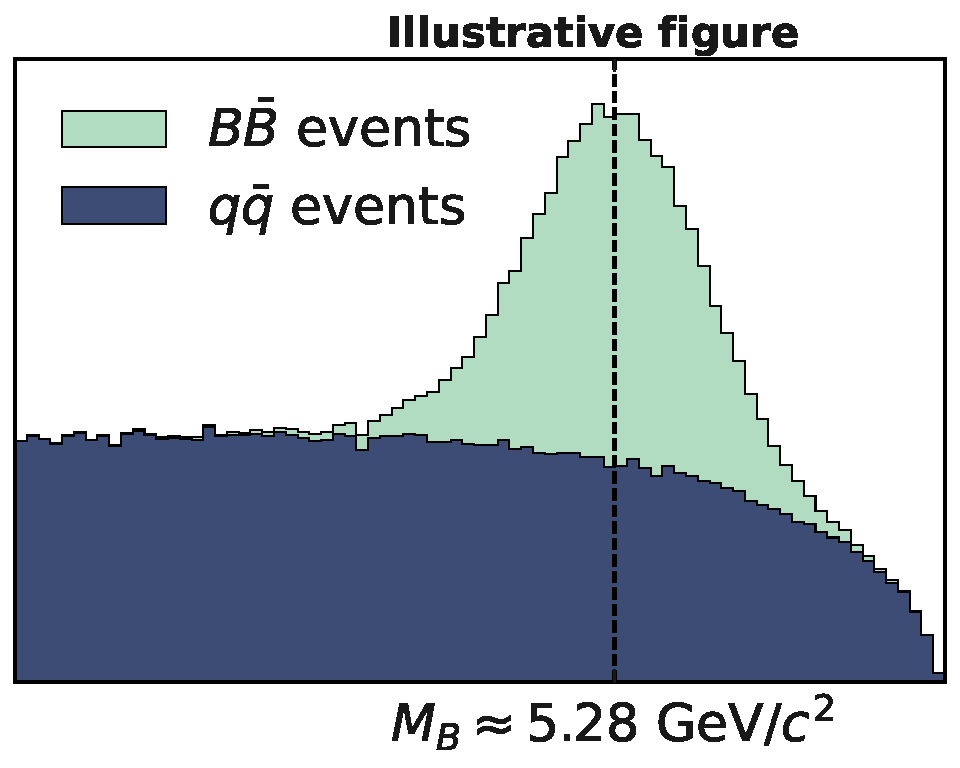
\includegraphics[width=0.72\textwidth]{figures/Mbc_mock_figure.pdf}
\end{columns}

\begin{tikzpicture} [remember picture, overlay]
   \node[rotate = 15] (t) at (0.5,1.35) {$\xrightarrow{\text{resonant-like behaviour}}$};
\end{tikzpicture}


\end{frame}

\begin{frame}{Reconstructed samples}
   \scriptsize
   \begin{itemize}
      \item \textbf{Because of hadronic tagging}, $B$ meson rest frame attainable
      \item[\ra] energy provided in the signal $B$ meson rest frame
      \item[\ra] \textbf{theoretically most desirable}!
      \item $\EB>1.4~\gev$ threshold adopted
      \item Only highest energy photon is selected
      % \item[\ra] compromise between disk space and maintaining as much signal as possible
      % \item Signal is modelled using a default Belle II model (Kagan-Neubert)

   \end{itemize}
   \begin{columns}
      \column{0.5\textwidth}
      \includegraphics[width=1\textwidth]{../phd_thesis/figures/event_reconstruction/Bp_tagged_background.pdf}
      \column{0.5\textwidth}
      \includegraphics[width=1\textwidth]{../phd_thesis/figures/event_reconstruction/Bz_tagged_background.pdf}
   \end{columns}
   \begin{itemize}
      \item[\ra] \textbf{non-}$\bm{\Upsilon(4S)}$ \textbf{processes dominant!}
   \end{itemize}
\end{frame}

\begin{frame}{Main photon background sources}
\centering\scriptsize

      % \begin{itemize}
      %    \item[\ra] Shown only for $B^+$ here, but similar for $B^0$
      % \end{itemize}

      \begin{tikzpicture}
         \node[] (img) at (0,0) {      \includegraphics[width=0.5\textwidth]{../phd_thesis/figures/event_selection/Bp_photon_sources.pdf}
         };
         \node[] (show) at (4.3,0.5) {
         \smash{\raisebox{.5\dimexpr1\baselineskip+2\itemsep+1\parskip}{$\left.\rule{0pt}{.35\dimexpr2\baselineskip+3\itemsep+3\parskip}\right\}\xrightarrow{\hspace*{0.3cm}}{\large\bm{0.5-3\%}\textbf{ each}}$}}
         };
         \node[] (showend) at (4.25,1.15) {
         \smash{\raisebox{.5\dimexpr1\baselineskip+2\itemsep+1\parskip}{$\left.\rule{0pt}{.3\dimexpr2\baselineskip+3\itemsep+3\parskip}\right\}\xrightarrow{\hspace*{1cm}}{\large\bm{85\%}\textbf{ of background}}$}}
         };

         % \draw [->,>=stealth] (show) -- (showend);

      \end{tikzpicture}

{\large \texttt{+}\textbf{about 4\% of misidentified photons}}

\end{frame}

\begin{frame}{Photon background suppression}
   \centering\scriptsize
   \begin{enumerate}
      \item {\bf\large\piz and $\eta$ suppression:}\\
      \item[\ra] \textbf{Combine all lower-energy photons with the high-energy photon candidate}
      \item[\ra] Use BDT to check for consistency with $\piz(\eta)\ra\g\g$\\
      \vspace{10pt}
      \item {\bf\large Mis-ID photon suppression:}\\
      \item[\ra] Photon and hadron showers differ in the electromagnetic calorimeter
      \item[\ra] Use BDT which combines photon calorimeter shower-shape paremeters 
  \end{enumerate}  
  \begin{columns}
   \column{0.33\textwidth}
   \includegraphics[width=1\textwidth]{../phd_thesis/figures/event_selection/Bp_piVeto.pdf}
   \column{0.335\textwidth}
   \includegraphics[width=1\textwidth]{../phd_thesis/figures/event_selection/Bz_etaVeto_nopi.pdf}
   \column{0.33\textwidth}
   \includegraphics[width=1\textwidth]{../phd_thesis/figures/event_selection/Bp_zernikeMVA_mcPDG.pdf}
\end{columns}

\begin{tikzpicture}[remember picture, overlay]
   \node[] (img) at (-3.5,2) {\bf\large 1};
   \node[] (img) at (1,2) {\bf\large 1};
   \node[] (img) at (5.5,2) {\bf\large 2};
\end{tikzpicture}

\end{frame}

% \begin{frame}{\piz and $\eta$ suppression}
%    \scriptsize\centering
% \begin{itemize}
%    \item $\piz\ra\g\g$ and $\eta\ra\g\g$ mimic the signal (high-$E$ $\gamma$ and low-$E$ $\gamma$)
%    \item \textbf{Combine all lower-energy photons with the high-energy photon candidate}
%    \item Evaluate the compatibility of the combination with a decay from \piz or $\eta$
%    \item[\ra] Use a BDT
% \end{itemize}
% \begin{columns}
%    \column{0.5\textwidth}
%    \includegraphics[width=1\textwidth]{../phd_thesis/figures/event_selection/Bp_piVeto.pdf}
%    \column{0.5\textwidth}
%    \includegraphics[width=1\textwidth]{../phd_thesis/figures/event_selection/Bz_etaVeto_nopi.pdf}
% \end{columns}

% \begin{flushright}
% \textbf{Standard approach implemented in the Belle~II software}
% \end{flushright}
% \end{frame}

% \begin{frame}{Photon misidentification}
% \centering   \scriptsize


% \begin{itemize}
%    \item Photon misidentification rate is small (96\% of photons are true photons)
%    \item Some hadrons leave clusters which are misidentified
% \end{itemize}

% \vspace{5pt}

% Multivariate tool, which parametrises the shower shape in terms of Zernike polynomial moments:

% \vspace{5pt}

% \includegraphics[width=0.5\textwidth]{../phd_thesis/figures/event_selection/Bp_zernikeMVA_mcPDG.pdf}


% \begin{flushright}
%    \textbf{Standard approach implemented in the Belle~II software}
%    \end{flushright}

% \end{frame}

\begin{frame}{Suppressing \qqbar events}
   \centering\scriptsize
   \begin{itemize}
      \item As seen at the beginning \textbf{many candidates originate in} {\boldmath$\epem\ra\qqbar$} \textbf{processes}
   \end{itemize}

   \includegraphics[width=0.5\textwidth]{../phd_thesis/figures/continuum_suppression/figure_continuum_suppression_event_shapes.pdf}

\begin{itemize}
\item $B$ factory experiments developed many ways to \textbf{parametrise the decay topology}
\item The parameters are combined using a \textbf{boosted decision tree}
\item \textbf{Problem:} decay topology is defined by particles in it 
\item[\ra] that \textbf{includes the $X_s$ system!}
% \item Every potential training feature is tested to not bias the photon energy spectrum!
% \item[\ra] 70 features tested \ra 26 final features used
\end{itemize}

\begin{tikzpicture}
   \node[] (img1) at (-3.5,0) {\includegraphics[width=0.35\textwidth]{../phd_thesis/figures/appendices/continuum_suppression_features/datamc_agreement_tests/Btag_cosTBz_agreement_tested.pdf}
   };
   \node[] (img2) at (3.5,0) {\includegraphics[width=0.35\textwidth]{../phd_thesis/figures/continuum_suppression/trained_bdtBDT_output_test.pdf}
   };
   \node[right= 0 cm of img1] (arrow1) {$\xrightarrow[\text{combined using a BDT}]{\text{26 \textbf{unbiasing} features}}$};

   % \draw[>,>=stealth] (arrow1) -- (arrow2);
\end{tikzpicture}

\end{frame}



% \begin{frame}{Continuum suppression training}
%    \scriptsize\centering
%    Converge to 26 training features, and evaluate the boosted decision tree training:

%    \begin{columns}
%       \column{0.5\textwidth}
%       \includegraphics[width=0.9\textwidth]{../phd_thesis/figures/continuum_suppression/roc_curve.png}
%       \includegraphics[width=0.9\textwidth]{../phd_thesis/figures/continuum_suppression/separation_curves.pdf}


%       % \column{0.5\textwidth}
%       % \includegraphics[width=0.9\textwidth]{../phd_thesis/figures/continuum_suppression/feature_importance.pdf}

%    \end{columns}
% \end{frame}

\begin{frame}{Selection optimisation}
\centering\scriptsize

\begin{itemize}
   \item The selections are optimised using a figure-of-merit and applied:
\end{itemize}

\vspace{5pt}

\begin{columns}
   \column{0.5\textwidth}
   \centering
   \includegraphics[width=0.85\textwidth]{../phd_thesis/figures/final_optimisation/Bp_tagged_background_optimal.pdf}
   \column{0.5\textwidth}
   \centering
   \includegraphics[width=0.85\textwidth]{../phd_thesis/figures/final_optimisation/Bz_tagged_background_optimal.pdf}
\end{columns}

\begin{itemize}
   \item[\ra] 100 times better signal-to-background ratio!
   \item After this point the tag side candidate with the highest \feiProb is picked
   \item[\ra] that leaves 1 tag + 1 photon candidate per event!
   \item[\ra] further background suppression by fitting
\end{itemize}

\end{frame}

\begin{frame}{Fitting the tag-side \Mbc distribution}
\scriptsize\centering

\begin{itemize}
   \item \textbf{Three tag categories} can be identified in the existing data samples
   \item They can be described by empirical parametric functions (PDFs)
   \item Example fits on the full dataset ($\EB>1.4~\gev$):
\end{itemize}

   \begin{columns}
      \column{0.33\textwidth}
      \centering
      {\color{ForestGreen} \epem\ra\BB good tags}
      \includegraphics[width=1\textwidth]{../phd_thesis/figures/fitting/mbc_good_tags_fit.pdf}

      \column{0.33\textwidth}
      \centering
      {\color{Bittersweet} \epem\ra\BB combinatorial}
      \includegraphics[width=1\textwidth]{../phd_thesis/figures/fitting/mbc_combinatorial_tags_fit.pdf}

      \column{0.33\textwidth}
      \centering
      {\color{Bittersweet} \epem\ra\qqbar events}
      \includegraphics[width=1\textwidth]{../phd_thesis/figures/fitting/mbc_continuum_tags_fit.pdf}

   \end{columns}

   \begin{itemize}
      \item [\ra] Use these PDFs to build a \textbf{total} $\bm{E_{\gamma}^B}$\textbf{-binned fitting model}
   \end{itemize}

   %  \begin{tikzpicture}[remember picture, overlay]
   %    \node[fill, white] (init) at (-5,5) {\color{black} discard};
   %    \node[] (inittwo) at (-4.6,4.9) {};
   %    \node[] (init2) at (-5,5.5) {accept};
      
   %    \node[] (end1) at (-4,5.2) {};
   %    \node[] (end2) at (-4,5.5) {};
   %    \node[] (end3) at (-4,4.8) {};
      
   %    \draw[-stealth] (init) -- (end1);
   %    \draw[-stealth] (inittwo) -- (end3);
   %    \draw[-stealth] (init2) -- (end2);
   %    \end{tikzpicture}
\end{frame}

\begin{frame}{Fit binning}
   \small\scriptsize\centering

   
   Optimal intervals based on statistical significance figure of merit studies:
   
   % \begin{itemize}
   %    \item 11 fitting intervals to extract \EB spectrum:\\
   %    \ra $1.4-1.8~\gev$ : two 200~\mev wide (control-region for fit)\\
   %    \ra $1.8-2.7~\gev$ : one 200~\mev and seven 100~\mev wide \textbf{(signal region)} \\
   %    \ra $2.7~\gev\mathtt{+}$  \hspace{14.5pt}: one `overflow' bin (control region for fit)\\
   %    \item The \textbf{fit is performed using the three PDFs} in every interval
   % \end{itemize}
   
   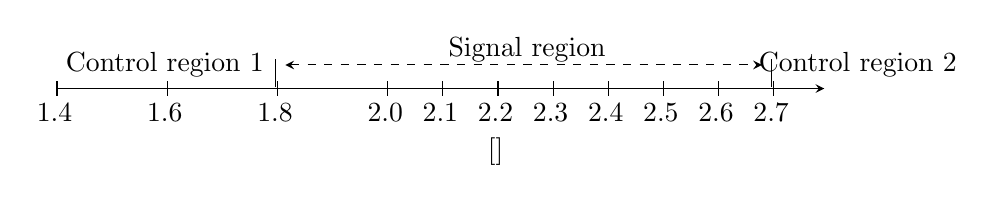
\begin{tikzpicture}
   \node[] (start) at (-5,0) {};
   \node[] (end) at (5,0) {};
   
   \node[] (1p6) at (-3.6,0) {};
   \node[] (1p8) at (-2.2,0) {};
   \node[] (2p0) at (-0.8,0) {};
   \node[] (2p1) at (-0.1,0) {};
   \node[] (2p2) at (0.6,0) {};
   \node[] (2p3) at (1.3,0) {};
   \node[] (2p4) at (2.0,0) {};
   \node[] (2p5) at (2.7,0) {};
   \node[] (2p6) at (3.4,0) {};
   \node[] (2p7) at (4.1,0) {};
   
   
   \draw[|->,>=stealth] (start)--(end);
   \draw[|-] (start)--(1p6);
   \draw[|-] (1p6)--(1p8);
   \draw[|-] (1p8)--(2p0);
   \draw[|-] (2p0)--(2p1);
   \draw[|-] (2p1)--(2p2);
   \draw[|-] (2p2)--(2p3);
   \draw[|-] (2p3)--(2p4);
   \draw[|-] (2p4)--(2p5);
   \draw[|-] (2p5)--(2p6);
   \draw[|-] (2p6)--(2p7);
   \draw[|-] (2p7)--(end);
   
   
   \node[] (starttext) at (-4.9,-0.3) {1.4};
   \node[] (endtext) at (4.9,-0.3) {};
   
   \node[] (1p6text) at (-3.5,-0.3) {1.6};
   \node[] (1p8text) at (-2.1,-0.3) {1.8};
   \node[] (2p0text) at (-0.7,-0.3) {2.0};
   \node[] (2p1text) at (-0.0,-0.3) {2.1};
   \node[] (2p2text) at (0.7,-0.3) {2.2};
   \node[] (2p3text) at (1.4,-0.3) {2.3};
   \node[] (2p4text) at (2.1,-0.3) {2.4};
   \node[] (2p5text) at (2.8,-0.3) {2.5};
   \node[] (2p6text) at (3.5,-0.3) {2.6};
   \node[] (2p7text) at (4.2,-0.3) {2.7};
   
   \node[] (sigregionstart) at (-2.093,0.3) {};
   \node[] (sigregionend) at (4.207,0.3) {};
   
   \node[] (sigregiondrawstart1) at (-2.093,-0.1) {};
   \node[] (sigregiondrawsend1) at (4.207,-0.1) {};
   \node[] (sigregiondrawstart2) at (-2.093,0.5) {};
   \node[] (sigregiondrawsend2) at (4.207,0.5) {};
   
   \node[] (sigregiontext) at (1.1,0.5) {Signal region};
   \node[] (cr1text) at (-3.5,0.3) {Control region 1};
   \node[] (cr2text) at (5.3,0.3) {Control region 2};
   
   
   \draw[<->,>=stealth,dashed] (sigregionstart) -- (sigregionend);
   \draw (sigregiondrawstart1) -- (sigregiondrawstart2);
   \draw (sigregiondrawsend1) -- (sigregiondrawsend2);

   \node[] (EB) at (0.7,-0.8) {\EB [$\gev$]};

   \end{tikzpicture}

   \vspace{5pt}
   
   Fits prepared on 1.6~\invab of simulation (four examples shown):


   \begin{columns}
      \column{0.5\textwidth}
      \centering
      \includegraphics[width=0.7\textwidth]{../phd_thesis/figures/fitting/fits/full_MbcFit_1p6to1p8ppdf.pdf}
      \includegraphics[width=0.7\textwidth]{../phd_thesis/figures/fitting/fits/full_MbcFit_2p0to2p1ppdf.pdf}
   
      \column{0.5\textwidth}
      \centering
      \includegraphics[width=0.7\textwidth]{../phd_thesis/figures/fitting/fits/full_MbcFit_2p3to2p4ppdf.pdf}
      \includegraphics[width=0.7\textwidth]{../phd_thesis/figures/fitting/fits/full_MbcFit_2p5to2p6ppdf.pdf}
   
   
   \end{columns}
   
   \begin{tikzpicture}[remember picture, overlay]
      \node[] at (0,3) (img) {\includegraphics[width=0.185\textwidth]{../phd_thesis/figures/fitting/legend.png}};
      \node[rectangle,
       draw = red,
       line width=0.5mm,
       minimum width = 2.2cm, 
       minimum height = 0.25cm] (r) at (0,2.42) {};
       \node[] at (0,2.0) {\tiny \color{red} $\mathcal{N}_{\mathrm{CB}}$: normalisation};
       \node[] at (0,1.8) {\tiny \color{red} $\equiv$ good tag count};

   \end{tikzpicture}
      
   \end{frame}

\begin{frame}{Fit validity on smaller data sets}
   \scriptsize\centering
   \begin{itemize}
      \item The analysis performed with 189~\invfb
      \item[\ra] test fitting stability on smaller data sample (1/10th)
   \end{itemize}

      \includegraphics[width=0.9\textwidth]{../phd_thesis/figures/mc_validation/extracted_signal_generic_mc.pdf}
  \begin{itemize}
   \item[\ra] irrespective of background levels, consistent fit result
   \item[\ra] But still the result does not look like a photon energy spectrum!   
  \end{itemize}

  \begin{itemize}
   \item Data sample of {\color{ForestGreen} good tags}:
\end{itemize}
    \textbf{(a)} \BtoXsgamma events + \textbf{(b)} remaining non-\BtoXsgamma background

\end{frame}

\begin{frame}{Remaining background}
\scriptsize\centering

       \vspace{10pt}
       \begin{itemize}
      \item Repeat the fit on \textbf{simulated background-only sample}
      \item[\ra] obtain only non-\BtoXsgamma background \textbf{and subtract}
      \item i.e. after unblinding:
   \end{itemize}
   \begin{equation*}
      N(\BtoXsdgamma) = \mathcal{N}_{\mathrm{CB}}(\text{Data}) - \mathcal{N}_{\mathrm{CB}}(\text{simulated background-only}) 
   \end{equation*}



   \includegraphics[width=0.9\textwidth]{../phd_thesis/figures/mc_validation/subtracted_signal_generic_mc.pdf}

\begin{itemize}
   \item[\ra] statistical uncertainty only, but clearly dominant 
\end{itemize}

\end{frame}




\begin{frame}{Simulation-to-data calibration}

   \scriptsize\centering
   
   \begin{itemize}
      \item Reliance on many different tools and background modelling
      \item Need to \textbf{ensure adequate agreement between data and simulation}
   \end{itemize}

   \vspace{10pt}

   Main supplementary calibration and modelling studies:

   \vspace{5pt}
   {\def\arraystretch{1.5}
\begin{tabular}{c|c|c}
   Calibration study & Method & Uncertainty \\
   \hline
   FEI & $B\to X \ell \nu$ & $\sim5\%$\\
   \piz and $\eta$ veto & $B^+\to \bar{D}^0\pi^+$ and $B^0\to D^-\pi^+$ & $\sim5-10\%$\\
   Photon detection efficiency &  $\epem\ra\mumu(\gamma)$ & \multirow{2}{*}{$\mathcal{O}(1\%)$}\\
   Post-fit background & world-average $\mathcal{B}$ variations & \\
\end{tabular}
   }
\vspace{10pt}

   \textbf{\ra henceforth, the application of these corrections is always assumed}

\end{frame}

\begin{frame}{Data-to-simulation validation}
   \scriptsize\centering
   \begin{columns}
      \column{0.5\textwidth}
      \centering
      
      Sample collected 60~\mev below the \FourS 
      
      (\textbf{only} $\bm{e^+e^-\rightarrow q\bar{q}}$)
      \includegraphics[width=0.75\textwidth]{../phd_thesis/figures/data_validation/Bboth_offresonance_EB.pdf}
      
      Sample with \texttt{BDT output} inverted 
      
      (\textbf{mostly} $\bm{e^+e^-\rightarrow q\bar{q}}$)
      \includegraphics[width=0.75\textwidth]{../phd_thesis/figures/data_validation/Bboth_qqbar_enhanced_eb.pdf}
      \column{0.5\textwidth}
      \centering
      
      Sample with $\piz$ and $\eta$ veto inverted 
      
      (\textbf{mostly} $\bm{B\bar{B}}$ \textbf{background})
      \includegraphics[width=0.75\textwidth]{../phd_thesis/figures/data_validation/Bboth_bbbar_enhanced_eb.pdf}
      
      Control regions 
      
      (\textbf{mostly} $\bm{B\bar{B}}$ \textbf{background})
      \includegraphics[width=0.75\textwidth]{../phd_thesis/figures/data_validation/Bboth_sidebands_eb.pdf}

   \end{columns}
\end{frame}

\begin{frame}{Normalisation discrepancy in the control regions}
\centering\scriptsize

   \includegraphics[width=0.55\textwidth]{../phd_thesis/figures/data_validation/Bboth_sidebands_eb.pdf}

   Two major culprits:
   \begin{itemize}
      \item Differences in \ZMVA behaviour (analysis specific background present)
      \item $\sqrt{s}$ variations in time affecting the $\epem\ra\qqbar$/$\epem\ra\FourS$ and \Mbc
      \item[] (not captured by data-taking period indpendent simulation)
   \end{itemize}

   \textbf{Both effects difficult to disentangle in this case}

   \ra apply a \textbf{conservative uncertainty} to cover background normalisation

\end{frame}

% \begin{frame}{Data-to-simulation validation: off-resonance sample}
% \scriptsize\centering
%    \begin{itemize}
%       \item Once appropriate corrections are calculated: validate the simulation using data
%       \item Using a sample collected 60~\mev below the \FourS
%       \item[\ra] $\epem\ra\qqbar$ validation
%    \end{itemize}
% \centering
%         \includegraphics[width=0.55\textwidth]{../phd_thesis/figures/data_validation/Bboth_offresonance_EB.pdf}

%         \begin{itemize}
%          \item[\ra] excellent \EB agreement
%          \item[\ra] however, off-resonance \Mbc is not comparable to on-resonance \Mbc
%         \end{itemize}

% \end{frame}

% \begin{frame}{Data-to-simulation validation: inverted continuum}
%    \scriptsize\centering
%    \begin{itemize}
%       \item Once appropriate corrections are calculated: validate the simulation using data
%       \item Flip \texttt{BDT output} of continuum suppression
%       \item[\ra]  $\epem\ra\qqbar$ validation with valid \Mbc
%    \end{itemize}

%    \begin{columns}
%       \column{0.5\textwidth}
%       \centering
%          \includegraphics[width=0.85\textwidth]{../phd_thesis/figures/data_validation/Bboth_qqbar_enhanced_eb.pdf}

%       \column{0.5\textwidth}
%       \centering
%          \includegraphics[width=0.85\textwidth]{../phd_thesis/figures/data_validation/Bboth_qqbar_enhanced_mbc.pdf}

%    \end{columns}

%    \begin{itemize}
%       \item Excellent agreement of \EB
%       \item Problematic for \Mbc!
%    \item[\ra] related to the fact that $\sqrt{s}$ may vary during data taking
%       \item[\ra] cannot be captured by data taking period independent simulation
%    \end{itemize}

% \end{frame}

% \begin{frame}{Data-to-simulation validation: inverted continuum}
%    \scriptsize\centering
%    \begin{itemize}
%       \item Once appropriate corrections are calculated: validate the simulation using data
%       \item Flip \texttt{BDT output} of continuum suppression
%       \item[\ra]  $\epem\ra\qqbar$ validation with valid \Mbc
%    \end{itemize}

%    \begin{columns}
%       \column{0.5\textwidth}
%       \centering
%          \includegraphics[width=0.85\textwidth]{../phd_thesis/figures/data_validation/Bboth_qqbar_enhanced_eb.pdf}
%       \column{0.5\textwidth}
%       \centering
%          \includegraphics[width=0.85\textwidth]{../phd_thesis/figures/data_validation/Bboth_qqbar_enhanced_mbccorrected.pdf}
%    \end{columns}

%    \begin{itemize}
%       \item Excellent agreement of \EB
%       \item Problematic for \Mbc!
%       \item[\ra] need to modify the \Mbc in simulation:  
%    \end{itemize}
%    \begin{equation*}
%       \sqrt{s}^{\mathrm{MC}} \xrightarrow[\mathrm{in~50\%~of~cases}]{\mathrm{replace~with~weighted~probability}} \sqrt{s}^{\mathrm{DATA}}
%    \end{equation*}

%    \begin{itemize}
%    \item[\ra] e.g. if x value is set for 30\% of data, then the weighted probability for x is 0.3
% \end{itemize}
% \end{frame}

% \begin{frame}{Data-to-simulation validation: inverted \piz and $\eta$}
%    \scriptsize\centering
%    \begin{itemize}
%       \item Once appropriate corrections are calculated: validate the simulation using data
%       \item Flip \piVeto and \etaVeto
%       \item[\ra]  $\BB$ background validation ($B\to X \piz$ and $B\to X \eta$)
%    \end{itemize}

%    \begin{columns}
%       \column{0.5\textwidth}
%       \includegraphics[width=0.85\textwidth]{../phd_thesis/figures/data_validation/Bboth_bbbar_enhanced_eb.pdf}
%       \column{0.5\textwidth}
%       \includegraphics[width=0.85\textwidth]{../phd_thesis/figures/data_validation/Bboth_bbbar_enhanced_mbccorrected.pdf}
%    \end{columns}

%    \begin{itemize}
%       \item Now only the `corrected' \Mbc is used!
%       \item Assign \textbf{the difference with, without corrected \Mbc as fit model uncertainty}!
%    \end{itemize}

% \end{frame}

% \begin{frame}{Data-to-simulation validation: sidebands}
%    \scriptsize\centering
%    \begin{itemize}
%       \item Once appropriate corrections are calculated: validate the simulation using data
%       \item The sideband region (\EB<1.8~\gev and \EB>2.7~\gev) with full signal selection
%    \end{itemize}

%    \begin{columns}
%       \column{0.5\textwidth}
%       \includegraphics[width=0.85\textwidth]{../phd_thesis/figures/data_validation/Bboth_sidebands_eb.pdf}
%       \column{0.5\textwidth}
%       \includegraphics[width=0.85\textwidth]{../phd_thesis/figures/data_validation/sidebands_mbc_1.pdf}
%    \end{columns}

%    \begin{itemize}
%       \item Now only the `corrected' \Mbc is used!
%       \item Not only \Mbc discrepancy but also endpoint discrepancy
%    \end{itemize}

% \end{frame}


\begin{frame}{Data-to-simulation validation: sidebands}
   \scriptsize\centering
   \begin{itemize}
      \item Similar behaviour observed after fitting:
   \end{itemize}

   \begin{columns}
      \column{0.33\textwidth}
      \centering
      \includegraphics[width=0.85\textwidth]{../phd_thesis/figures/data_validation/sidebands_fit/DATA_MbcFit_1p4to1p6ppdf.pdf}
      \column{0.33\textwidth}
      \centering
      \includegraphics[width=0.85\textwidth]{../phd_thesis/figures/data_validation/sidebands_fit/DATA_MbcFit_1p6to1p8ppdf.pdf}
      \column{0.33\textwidth}
      \centering
      \includegraphics[width=0.85\textwidth]{../phd_thesis/figures/data_validation/sidebands_fit/DATA_MbcFit_2p7to5p0ppdf.pdf}
   \end{columns}

   \begin{itemize}
      \item $\mathcal{N}_{\mathrm{DATA}}/\mathcal{N}_{\mathrm{MC}}\approx 1.087\pm 0.080$
   \end{itemize}

   \includegraphics[width=0.45\textwidth]{../phd_thesis/figures/data_validation/sidebands_background_vs_data.pdf}

\end{frame}
\begin{frame}{Data-to-simulation validation: sidebands}
   \scriptsize\centering
   \begin{itemize}
      \item Or the same with background subtracted:
   \end{itemize}

   \begin{columns}
      \column{0.5\textwidth}
      \centering
      \includegraphics[width=0.85\textwidth]{../phd_thesis/figures/data_validation/sideband_event_counts.pdf}
    \column{0.5\textwidth}
    \centering
     \includegraphics[width=0.85\textwidth]{../phd_thesis/figures/data_validation/sideband_event_counts_corrected.pdf}
   \end{columns}

   $\xrightarrow{\text{Apply an 8.7\% correction, because we expect the results here to be consistent with 0}}$

   \begin{itemize}
      \item Assign \textbf{the full correction as a systematic uncertainty}
      \item[\ra] Conservative approach: also accommodates the issues seen earlier
      \item[\ra] Dominant uncertainty (normalisation of background)!
   \end{itemize}

\end{frame}

\begin{frame}{\BtoXsgamma efficiency validation}
\scriptsize\centering
\begin{itemize}
   \item Efficiency is assumed to factorise:
\end{itemize}
\begin{equation*}
   \varepsilon_{\BtoXsgamma} = \varepsilon_{\mathrm{FEI}} \cdot \varepsilon_{\mathrm{selection}}
\end{equation*}

\vspace{-5pt}

\begin{itemize}
   \item $\varepsilon_{\mathrm{FEI}}$ calculated \textbf{based on simulation + corrected}:
\end{itemize}
\begin{equation*}
   \varepsilon_{\mathrm{FEI}} = (0.444\pm0.015) \%
\end{equation*}

\vspace{-5pt}

\begin{itemize}
   \item $\varepsilon_{\mathrm{selection}}$ are calculated \textbf{based on simulation + corrected}:
   \begin{itemize}
      \scriptsize
      \item \piVeto and \etaVeto correction, photon detection efficiency 
      \vspace{5pt}
      \item \texttt{BDToutput}, \texttt{ZernikeMVA} by varying their selection 
      \item[\ra] variations directly in data (blinded) evaluated and assigned as uncertainty
   \end{itemize}
\end{itemize}
\begin{tikzpicture}
   \node[] (img) at (0,0) {\includegraphics[width=0.45\textwidth]{../phd_thesis/figures/signal_validation/corrected_selection_efficiency.pdf}
   };
   \node[] (img) at (4,0) {$\approx 10\%$ uncertainty};
\end{tikzpicture}

\end{frame}

\begin{frame}{Unfolding}
\centering\scriptsize

\begin{itemize}
   \centering
   \item[] Real phenomenon $\xrightarrow{\textbf{measurement}}$ measured results
   \item[] Measured results $\xrightarrow[\text{model reliant}]{\textbf{unfolding}}$ `real phenomenon'

\end{itemize}
\begin{itemize}
   \item[\ra] Detector modelling encoded in Belle~II simulation software
   \item \textbf{Bin-by-bin correction} - simplest approach, acceptable due to large statistical uncertainty
\end{itemize}
\begin{equation*}
   \mathcal{U}_i = \frac{N(\BtoXsgamma)_{\text{generated},i}}{N(\BtoXsgamma)_{\text{measured},i}}~\text{for a given \EB interval}~i
\end{equation*}
% \begin{equation*}\label{eq:bin_by_bin_unfolding}
%    x_i = y_i \cdot \frac{N_i^{\mathrm{gen}}}{N_i^{\mathrm{meas}}},
%   \end{equation*}

%   \begin{equation*}\label{eq:bin_by_bin_unfolding_error}
%       \Delta x_i = \Delta y_i \cdot \frac{N_i^{\mathrm{gen}}}{N_i^{\mathrm{meas}}},
%   \end{equation*}
\begin{itemize}
   \item Unfolding model for evaluating $N(\BtoXsgamma)$:
   \item[\ra] inclusive \BtoXsgamma model with
   \item[+] $B\to\Kstar(892)\gamma$ resonance
\end{itemize}

\begin{columns}
   \column{0.5\textwidth}
   \centering
   \textbf{Model:}
   \includegraphics[width=0.85\textwidth]{../phd_thesis/figures/data_samples/normalised_signal_model.pdf}

   \column{0.5\textwidth}
   \centering
   \textbf{Unfolding} (simulation):
   \includegraphics[width=0.85\textwidth]{../phd_thesis/figures/signal_validation/reco_vs_true_spectrum.pdf}

\end{columns}


\end{frame}

% \begin{frame}{Systematic uncertainties}
%    \scriptsize\centering
%    \begin{itemize}
%       \item Summary of systematic uncertainties that are evaluates:
%       \item[\ra] Background modelling/normalisation uncertainties
%       \item[\ra] Fit model uncertainties
%       \item[\ra] Efficiency uncertainties
%       \item[\ra] Unfolding and \BtoXdgamma uncertainties   
%    \end{itemize}
% \end{frame}

\addtocounter{framenumber}{-1}
{\setbeamertemplate{footline}{} 
\begin{frame}
   \centering
   \textbf{Unblinded results}
\end{frame}
}

\begin{frame}{Fit results}
\begin{columns}
   \column{0.33\textwidth}
   \centering
   \includegraphics[width=1\textwidth]{../phd_thesis/figures/final_results/data_fits/DATA_MbcFit_1p8to2p0ppdf.pdf}
   \includegraphics[width=1\textwidth]{../phd_thesis/figures/final_results/data_fits/DATA_MbcFit_2p2to2p3ppdf.pdf}

   \column{0.33\textwidth}
   \centering
   \includegraphics[width=1\textwidth]{../phd_thesis/figures/final_results/data_fits/DATA_MbcFit_2p0to2p1ppdf.pdf}
   \includegraphics[width=1\textwidth]{../phd_thesis/figures/final_results/data_fits/DATA_MbcFit_2p3to2p4ppdf.pdf}

   \column{0.33\textwidth}
   \centering
   \includegraphics[width=1\textwidth]{../phd_thesis/figures/final_results/data_fits/DATA_MbcFit_2p1to2p2ppdf.pdf}
   \includegraphics[width=1\textwidth]{../phd_thesis/figures/final_results/data_fits/DATA_MbcFit_2p4to2p5ppdf.pdf}
\end{columns}
\begin{columns}
   \column{0.5\textwidth}
   \centering
   \includegraphics[width=0.66\textwidth]{../phd_thesis/figures/final_results/data_fits/DATA_MbcFit_2p5to2p6ppdf.pdf}
   \column{0.5\textwidth}
   \centering
   \includegraphics[width=0.66\textwidth]{../phd_thesis/figures/final_results/data_fits/DATA_MbcFit_2p6to2p7ppdf.pdf}

\end{columns}
\end{frame}



\begin{frame}{Background subtracted results}
   \centering\scriptsize
\textbf{Fit results summarised:}

   \includegraphics[width=0.45\textwidth]{../phd_thesis/figures/final_results/background_vs_data_final.pdf}
   % \column{0.5\textwidth}
   % \centering
   % \includegraphics[width=0.85\textwidth]{../phd_thesis/figures/final_results/background_vs_data_final_log.pdf}

\textbf{Background subtracted:}

\vspace{-3pt}

   \centering
   \begin{tikzpicture}
      \node[] (img1) at (0,0) {      \includegraphics[width=0.45\textwidth]{../phd_thesis/figures/final_results/reco_spectrum_overlayed_signal_region.pdf}
      };
      \node[] (img2) at (0.25,1.3) {      \clipbox*{{0.62\width} {0.56\height} {0.88\width} {0.68\height}}{
         \includegraphics[width=0.45\textwidth]{../phd_thesis/figures/final_results/reco_spectrum_overlayed.pdf}
      }
      };
      \node[] (img3) at (1.8,1.3) {      \clipbox*{{0.6\width} {0.41\height} {0.895\width} {0.56\height}}{
         \includegraphics[width=0.45\textwidth]{../phd_thesis/figures/final_results/reco_spectrum_overlayed.pdf}
      }
      };
 
   \end{tikzpicture}


\end{frame}

\begin{frame}{Total and partial branching fractions}
   \centering\scriptsize
      \includegraphics[width=0.45\textwidth]{../phd_thesis/figures/final_results/partial_bfs.pdf}

      \textbf{Or numerically:}
      \vspace{5pt}

      \resizebox{1\textwidth}{!}{
         \begin{tabular}{|c|ccc||cccc|}
         \hline
         \multirow{2}{*}[-6pt]{\EB interval [\gev]} &
         \multirow{2}{*}[-6pt]{$\frac{\Delta\mathcal{B}(\BtoXsgamma)_i}{\Delta {E^B_{\g}}_{,i}} (10^{-4})$} &
         \multirow{2}{*}[-6pt]{\makecell{Statistical\\uncertainty} ($10^{-4}$)} &
         \multirow{2}{*}[-6pt]{\makecell{Systematic\\uncertainty} ($10^{-4}$)}& 
         \multicolumn{4}{c|}{Systematic uncertainty group} \\
         \cline{5-8}
         & & & &        
         \makecell{Background \\ modelling} &
         \makecell{\Mbc fit \\ model} & 
         \makecell{\BtoXsgamma \\efficiency} & 
         \makecell{Other\\uncertainties}\\
         \hline
         $1.8-2.0$  &  0.48 & $\pm0.54$ & $\pm0.64$ & 0.49 & 0.42 & 0.03 & 0.09 \\
         $2.0-2.1$  &  0.57 & $\pm0.31$ & $\pm0.25$ & 0.17 & 0.17 & 0.06 & 0.07 \\
         $2.1-2.2$  &  0.13 & $\pm0.26$ & $\pm0.16$ & 0.11 & 0.13 & 0.01 & 0.01 \\
         $2.2-2.3$  &  0.41 & $\pm0.22$ & $\pm0.10$ & 0.04 & 0.07 & 0.05 & 0.02 \\
         $2.3-2.4$  &  0.48 & $\pm0.22$ & $\pm0.10$ & 0.02 & 0.06 & 0.06 & 0.05 \\
         $2.4-2.5$  &  0.75 & $\pm0.19$ & $\pm0.14$ & 0.02 & 0.04 & 0.09 & 0.09 \\
         $2.5-2.6$  &  0.71 & $\pm0.13$ & $\pm0.10$ & 0.00 & 0.02 & 0.09 & 0.04  \\
         \hline
         \end{tabular}
     }
\begin{itemize}
   \item Other uncertainties: 
   \item[] subtraction of \BtoXdgamma component, unfolding, uncertainty of $B$ mesons in the sample
\end{itemize}
\end{frame}

\begin{frame}{Integrated branching fraction: comparison}
\centering\scriptsize

\begin{itemize}
   \item Sum of the photon energy spectrum:
\end{itemize}
\begin{itemize}
   \centering
   \item[$\EB>1.8~\gev$] $\mathcal{B}(\BtoXsgamma) = (3.54 \pm 0.78~(\text{stat.}) \pm 0.83~(\text{syst.}))\times 10^{-4}$ \\
\end{itemize}

\begin{itemize}
   \item Compare with BaBar hadronic-tagged result:
\end{itemize}
\begin{itemize}
   \centering
   \item[$\EB>1.9~\gev$]  $\mathcal{B}(\BtoXsgamma) = (3.66 \pm 0.85~(\text{stat.}) \pm 0.60~(\text{syst.}))\times 10^{-4}$ \\
\end{itemize}

\vspace{10pt}

Comparison of all results: (Extrapolation to $\EB>1.6~\gev$)

      \includegraphics[width=0.7\textwidth]{../phd_thesis/figures/results_discussion/all_measurements_compared.pdf}


      
\end{frame}

    


\begin{frame}{Input to the theoretical calculations (SIMBA collaboration)}
\centering\scriptsize

\vspace{10pt}

\begin{columns}
   \centering
   \column{0.5\textwidth}
   \centering\scriptsize

   \includegraphics[width=0.45\textwidth]{figures/babar_hadtag_spec_default_la055_a3.pdf}
   \includegraphics[width=0.45\textwidth]{figures/babar_incl_spec_default_la055_a3.pdf}
   \includegraphics[width=0.45\textwidth]{figures/babar_sem_spec_default_la055_a3.pdf}
   \includegraphics[width=0.45\textwidth]{figures/belle_spec_default_la055_a3.pdf}
   
   {\Large + this work}
   
   \includegraphics[width=0.85\textwidth]{../phd_thesis/figures/results_discussion/simba_partial_bfs_expectation.pdf}

   \column{0.5\textwidth}
   \centering
   \begin{itemize}
      \item[]          {\tiny\textbf{Phys.Rev.Lett. 127 (2021) 10, 102001}}
      \item Exact interpretation of the photon energy spectrum and $\mathcal{F}$ is model dependent
      \item \textbf{Global fit of all experimental information}
      \item Extract spectrum normalisation, shape function parameters (e.g. $m_b$)
   \end{itemize}
   \includegraphics[width=0.85\textwidth]{../phd_thesis/figures/results_discussion/C7incl_mb_la055_henrikas.pdf}

\end{columns}

\begin{tikzpicture}[remember picture, overlay]
   \node (dog) at (-0.19,3.7) {\LARGE $\bm{\Longrightarrow}$};
   \node (dogbackup1) at (0.5,0.7) {normalisation};
   \node (dogbackup2) at (-0.3,6.2) {};
   \node (catbackup1) at (0.8,2.15) {};
   \node (catbackup2) at (0.6,6.2) {};

   \draw[->,>=stealth, color=red] (dogbackup1) -- (catbackup1);
   \draw[->,>=stealth, color=red] (catbackup2) -- (dogbackup2);

   \node (catbackup3) at (-3.,8.2) {\textbf{BaBar and Belle results}};

\end{tikzpicture}

\end{frame}   

\begin{frame}{Outlook and summary}
\scriptsize


{\small \textbf{Summary}}


   \begin{itemize}
      \item \BtoXsgamma \textbf{photon energy spectrum} and \textbf{total decay rate} measured
      \item \textbf{Hadronic tagging} technique implemented!
      \item[\ra] It is the \textbf{first such measurement at Belle II and Belle}
      \item[] (and second ever, overall)
      \item \textbf{Sets the stage} for future hadronic-tagged \BtoXsgamma measurements at Belle~II
   \end{itemize}

   \vspace{15pt}

   {\small \textbf{Outlook} for \BtoXsgamma}

   \begin{itemize}
      \item Quite a few other measurement techniques are already limited systematically\\
      \item \textbf{Hadronic-tagged analysis only limited at $1-10$~\invab}\\
      \begin{flushright}
         \tiny
         \textbf{Snowmass White Paper: Belle II physics reach and plans for the next decade and beyond}
      
      e-Print: 2207.06307 [hep-ex]
      \end{flushright}
      \item Results are awaited by the theory community as well 
      \item[\ra] \textbf{important for the Standard Model and beyond}
   \end{itemize}




\end{frame}

\appendix

%----------------------------------------------------------------------------------------
%	B to Xs gamma
%----------------------------------------------------------------------------------------
\section{Appendix}

\begin{frame}{\hypertarget{frame:A}{Appendix}}

   \centering\scriptsize

   \tableofcontents

\end{frame}

\section{Theoretical description}

\begin{frame}{Description of the inclusive decays \hyperlink{frame:A}{$\circlearrowleft$}}
   \scriptsize

   \begin{itemize}
      \item Fully inclusive decay rate is related to the \textbf{the parton decay rate}
      \item The $b\to s$ electroweak loop is \textbf{dominated by the top quark} 
      \item It \textbf{involves both weak and strong interactions}
      \item[\ra] energy scale $\ll\order(m_W)$
      \item[\ra] approximate weak interactions with effective point-like vertices.
   \end{itemize}

   \textbf{Effective Lagrangian:}
   \begin{equation}\nonumber
      \mathcal{L}_{\mathrm{eff}} = \frac{4G_F}{\sqrt{2}}V_{tq}^*V_{tb}\left[\sum^{8}_{i=1}\mathcal{C}_i(\mu)\mathcal{O}_i(\mu)
                                                  + \frac{V^*_{uq}V_{ub}}{V^*_{tq}V_{tb}}\sum^{2}_{i=1}\mathcal{C}_i(\mu)(\mathcal{O}_i(\mu)-\mathcal{O}_i^u(\mu))\right]
  \end{equation}

  \vspace{10pt}

  $\mathcal{C}_i$: Wilson coefficients (encode \Wpm, $Z$ and $t$ interactions)
  
  $\mathcal{O}_i$: Four-quark and dipole-type operators (quark interactions)

\end{frame}

\begin{frame}{Description of the inclusive decays\hyperlink{frame:A}{$\circlearrowleft$}}
   \scriptsize

   \begin{equation}\nonumber
      \mathcal{L}_{\mathrm{eff}} = \frac{4G_F}{\sqrt{2}}V_{tq}^*V_{tb}\left[\sum^{8}_{i=1}\mathcal{C}_i(\mu)\mathcal{O}_i(\mu)
                                                  + {\underbrace{\frac{V^*_{uq}V_{ub}}{V^*_{tq}V_{tb}}}_{\substack{\approx 0.02,~\mathbf{q = s}\\\approx 0.47,~\mathbf{q = d}}}}\sum^{2}_{i=1}\mathcal{C}_i(\mu)(\mathcal{O}_i(\mu)-\mathcal{O}_i^u(\mu))\right]
   \end{equation}

\begin{itemize}
   \item For \btosgamma the second term is much less important
   \item It is relevant for higher order corrections, and for \btodgamma
\end{itemize}

\end{frame}


\begin{frame}{\safeBtoXsgamma total decay rate calculations\hyperlink{frame:A}{$\circlearrowleft$}}
\scriptsize
   \begin{itemize}
      \item That was for the \textit{parton} decay rate;
      \item[\ra] can be calculated perturbatively 
      \item Switch from partons to hadrons assuming quark-hadron duality:
   \end{itemize}

   \vspace{10pt}

   \begin{equation}\nonumber
      \Gamma(B\ra\X_s\g) = \Gamma(b\ra s\g) + \underbrace{\Delta\Gamma_{\mathrm{non-p.}}}_{\substack{\text{additional}\\\text{non-perturbative}\\\text{term}}}
  \end{equation}
  \begin{itemize}
   \item[\ra] related to the fact that the $b$ quark is non-stationary and within a $B$ meson
   \item Many such effects decrease or `average out' over the totality of the spectrum
   \item However, others remain: e.g. around $\Egamma<1.5~\gev$ non-perturbative \ccbar contributions become relevant 
     \end{itemize}

     \textbf{A convention $\Egamma>1.6~\gev$ chosen in inclusive decay rate calculations}

\end{frame}

\section{\safeBtoXsgamma spectrum description}


\begin{frame}{\safeBtoXsdgamma spectrum calculations\hyperlink{frame:A}{$\circlearrowleft$}}
\scriptsize
   Non-perturbative effects more complicated if the partial decay rates are considered

   \begin{columns}
      \column{0.5\textwidth}
      \includegraphics[width=1\textwidth]{../phd_thesis/figures/theory/xsgamma_theory_to_experiment.png}
      \column{0.5\textwidth}
      \includegraphics[width=1\textwidth]{../phd_thesis/figures/theory/xsgamma_theory_components.png}
   \end{columns}

   \begin{itemize}
      \item Use soft-collinear effective field theory:
   \end{itemize}
   \begin{equation}\nonumber
      d\Gamma \propto \mathcal{H} \times \mathcal{J} \otimes \mathcal{S}.
  \end{equation}
  which splits the calculation of:
  \begin{itemize}
   \item[] {\color{red}$\mathcal{H}$: effective hard interaction (perturbative)}
   \item[] {\color{blue}$\mathcal{J}$: collinear particle interactions (perturbative)}
   \item[] {\color{orange}$\mathcal{S}$: soft particle interactions}
  \end{itemize}

\vspace{-10pt}

\begin{flushright}
   \tiny \textbf{Credit to Frank Tackmann for the illustrations.}
\end{flushright}

\end{frame}

\begin{frame}{\safeBtoXsdgamma spectrum calculations\hyperlink{frame:A}{$\circlearrowleft$}}
   \scriptsize
      Non-perturbative effects more complicated if the partial decay rates are considered
   
      \begin{columns}
         \column{0.5\textwidth}
         \includegraphics[width=1\textwidth]{../phd_thesis/figures/theory/xsgamma_theory_to_experiment.png}
         \column{0.5\textwidth}
         \includegraphics[width=1\textwidth]{../phd_thesis/figures/theory/xsgamma_theory_components.png}
      \end{columns}
   
      \begin{itemize}
         \item Use soft-collinear effective field theory:
      \end{itemize}
      \begin{equation}\nonumber
         d\Gamma \propto \mathcal{H} \times \mathcal{J} \otimes \mathcal{S}.
     \end{equation}

     \vspace{-10pt}
     \begin{itemize}
      \item It is assumed that:
     \end{itemize}
     \begin{equation}\nonumber
      \mathcal{S} \equiv \underbrace{\mathcal{S}_p}_{\substack{\text{perturbative}\\\text{partonic soft function}}} \otimes \underbrace{\mathcal{F}}_{\substack{\text{non perturbative}\\\textbf{shape function}}}
     \end{equation}
     \begin{itemize}
      \item[\ra] the theory is capable to separate perturbative and non-perturbative terms 
     \end{itemize}

   \vspace{-5pt}
   
   \begin{flushright}
      \tiny \textbf{Credit to Frank Tackmann for the illustrations.}
   \end{flushright}
   
   \end{frame}


   \begin{frame}{\BtoXsgamma spectrum and the shape function\hyperlink{frame:A}{$\circlearrowleft$}}
      \scriptsize
      \begin{itemize}
         \item The shape function $\mathcal{F}$ encodes the Fermi motion of the $b$ and is therefore \textbf{universal for the} \bm{$B$} \textbf{meson}\footnote[1]{\tiny however, more shape function need to be introduced at higher orders}
         \item \textbf{Crucial input for other analyses}, e.g. $|V_{ub}|$ measurements with $B\to\X_u\ell\nu$, using phase space selection to separate $B\to\X_c\ell\nu$ states
      \end{itemize}

      \textbf{So how to evaluate it?}
      \begin{itemize}
         \item[\ra] you have to use experimental information: 
         \item[\ra] \BtoXsgamma is a highly suitable channel for this
      \end{itemize}

   \end{frame}

   \begin{frame}{\BtoXsgamma spectrum and the shape function\hyperlink{frame:A}{$\circlearrowleft$}}
      \scriptsize
      It can be shown that the moments of photon energy spectrum relate to
      \begin{equation}\nonumber
         \expval**{\Egamma} \sim m_b/2+\order(\Lambda_{\mathrm{QCD}}); \quad \expval**{\Egamma^2}-\expval**{\Egamma}^2 \sim \lambda_1/12+\order(\Lambda_{\mathrm{QCD}}),
     \end{equation}
     with:
     \begin{itemize}
      \item [] $m_b$: $b$ quark pole mass
      \item [] $\lambda_1$: $b$ quark kinetic energy parameter
      \item [] etc. for higher moments
     \end{itemize}
   $\mathcal{F}$ can be parametrised in terms of these quantities!
   \end{frame}

   \section{Kagan-Neubert model}


   \begin{frame}{Kagan-Neubert model}
      \scriptsize
      \textbf{Kagan-Neubert} model is often used for experimental analyses:
      \begin{equation}\nonumber
         \mathcal{F}(x) = N\left(1-\frac{x}{m_B-m_b}\right)^a\exp{(1+a)\frac{x}{m_B-m_b}},
     \end{equation}

     where $a$ is related to the second moment of $\mathcal{F}$:
     \begin{equation*}
      A_2 = \frac{m_B-m_b}{1+a} \quad A_2 \equiv -\lambda_1/3
     \end{equation*}


     Then the spectrum can be described by two parameters: $m_b$ and $\lambda_1$;

     \begin{center}

     \includegraphics[width=0.5\textwidth]{figures/kagan_neubert.png}
   \end{center}
   \end{frame}

   \section{BSM physics in \safeBtoXsgamma}


\begin{frame}{Beyond the Standard Model \hyperlink{frame:A}{$\circlearrowleft$}}
   \scriptsize
   Only heavy particles are expected, in other words, the effective Lagrangian would be modified as:
   \begin{equation}\nonumber
      \mathcal{C}_i^{\mathrm{SM}} \ra \mathcal{C}_i^{\mathrm{SM}} + \Delta\mathcal{C}_i^{\mathrm{BSM}}.
   \end{equation}
   Some models may propose $\Delta\mathcal{C}_j^{\mathrm{BSM}}$, where $\mathcal{C}_j^{\mathrm{SM}}=0$

\vspace{10pt}
   In no particular order, some (but surely not all) theories which propose such modifications:
   \begin{itemize}
      \item two-Higgs-doublet models 
      \item[\ra] more in next slides
      \item minimal supersymmetric models with minimal flavour violation
      \item[\ra] flavour violation only in CKM
      \item left-right symmetric models
      \item general minimal-supersymmetric theories
      \item models with extra dimensions
      \item the littlest Higgs models
      \item 331 models
   \end{itemize}
\end{frame}

\begin{frame}{Two-Higgs-doublet models \hyperlink{frame:A}{$\circlearrowleft$}}

   \scriptsize

   \textbf{New term in the SM Lagrangian:}
   \begin{equation*}
      \mathcal{L}_{H^+} = \frac{1}{\sqrt{\sqrt8G_F}} \sum_{i,j=1} \bar{u}_i (A_u m_{u_i}V_{ij}P_L - A_d m_{d_j}V_{ij}P_R)d_jH^+ + \mathrm{h.c}.
  \end{equation*}

  \textbf{Couplings:}

\begin{align*}
A_u = A_d = \frac{1}{\tan\beta} \quad (\textbf{type I})\\
A_u = - \frac{1}{A_d} = \frac{1}{\tan\beta} \quad  (\textbf{type II})
\end{align*}

\textbf{Wilson coefficients:}

\begin{equation*}\label{eq:partial_wilson_2hdm}
   \Delta C_i^{(0)\text{2HDM}} = 
   \begin{cases}
       0, & i=1,...,6;\\
       \frac{A_u^2}{3}F_i^{(1)}(y) - A_uA_dF_i^{(2)}(y), & i=7,8;\\
   \end{cases}
\end{equation*}
and $y = m_t/m_{H^+}$
\end{frame}

\begin{frame}{Two-Higgs-Doublet models}
   \centering
\begin{columns}
   \column{0.5\textwidth}
   \includegraphics[width=0.9\textwidth]{../phd_thesis/figures/theory/xsgamma_2hdm_type1.png}
   \column{0.5\textwidth}
   \includegraphics[width=0.9\textwidth]{../phd_thesis/figures/theory/xsgamma_2hdm_type2.png}
\end{columns}

       \includegraphics[width=0.5\textwidth]{../phd_thesis/figures/theory/xsgamma_2hdm_both_types.png}


  
\end{frame}

\section{Belle II}


\begin{frame}{Pixel vertex detector \hyperlink{frame:A}{$\circlearrowleft$}}

   \scriptsize

   \begin{columns}
      \column{0.5\textwidth}
      \centering
         \includegraphics[width=0.7\textwidth]{../phd_thesis_defense_slides/figures/pxd_efficiency.png}
      \column{0.5\textwidth}
      \centering
         \includegraphics[width=0.7\textwidth]{../phd_thesis_defense_slides/figures/pxd_layers.png}
   \end{columns}

   \begin{columns}
      \column{0.5\textwidth}
      \centering
         \includegraphics[width=0.7\textwidth]{../phd_thesis_defense_slides/figures/pxd_depfet.png}
      \column{0.5\textwidth}
         \begin{itemize}
            \item DEPFET technology
            \item Hit efficiency ~99\% in good regions
            \item $z$ resolution $\sim15~\si{\micro\meter}$
         \end{itemize}
         {\tiny\textbf{Nuclear Inst. and Methods in Physics Research, A 1032 (2022) 166631}}
   \end{columns}
\end{frame}

\begin{frame}{Silicon vertex detector \hyperlink{frame:A}{$\circlearrowleft$}}
\centering\scriptsize

Double Sided Silicon Strip sensors:
\vspace{10pt}

   \begin{columns}
      \column{0.5\textwidth}
      \centering
      \includegraphics[width=0.8\textwidth]{../phd_thesis/figures/experimental_setup/vxd.png}
      \column{0.5\textwidth}
      \centering
      \includegraphics[width=0.8\textwidth]{figures/svd_details.png}

   \end{columns}

   \vspace{10pt}

   \includegraphics[width=0.8\textwidth]{figures/svd_resolution.png}

   \begin{flushright}
   \tiny\textbf{Nuclear Inst. and Methods in Physics Research, A 1045 (2023) 167578}
   \end{flushright}
\end{frame}

\begin{frame}{Central drift chamber \hyperlink{frame:A}{$\circlearrowleft$}}
   \centering\scriptsize
   \begin{columns}
      \column{0.5\textwidth}
      \centering
      \includegraphics[width=0.7\textwidth]{../phd_thesis/figures/experimental_setup/cdc_quadrant.png}
      \column{0.5\textwidth}
      \centering
      \includegraphics[width=0.7\textwidth]{../phd_thesis/figures/experimental_setup/cdc_layers.png}
   \end{columns}

   \begin{columns}
      \column{0.5\textwidth}
      \centering
         \includegraphics[width=0.8\textwidth]{figures/cdc_resolution.png}
      \column{0.5\textwidth}
      \begin{itemize}
         \item 56 layers: axial and stereo orientation
         \item $0.1-0.2$ cm resolution
         \item He-C$_2$H$_6$ gas mixture
      \end{itemize}

      \begin{flushright}
        \tiny \textbf{e-Print: 1910.06289 [physics.ins-det]}
      \end{flushright}
      
   \end{columns}


\end{frame}

\begin{frame}{Particle identification systems \hyperlink{frame:A}{$\circlearrowleft$}}
   \scriptsize
   \begin{columns}
      \column{0.5\textwidth}
      \centering
      \textbf{Time of propagation counter}
         \includegraphics[width=0.9\textwidth]{figures/top_schematic.png}
         \begin{itemize}
            \item 85\% $K^{\pm}$ identification at 10\% $\pi^{\pm}$ misidentification
         \end{itemize}
      \column{0.5\textwidth}
      \textbf{Ring-imaging Cherenkov counter}
         \includegraphics[width=0.9\textwidth]{figures/arich_schematic.png}
         \begin{itemize}
            \item 94\% $K^{\pm}$ identification at 11\% $\pi^{\pm}$ misidentification
         \end{itemize}
   \end{columns}
   \begin{flushright}
     \tiny \textbf{PoS EPS-HEP2021 (2022), 803}

      \tiny \textbf{PTEP 2020 (2020) 9, 093H01}
   \end{flushright}
\end{frame}

\begin{frame}{Electromagnetic calorimeter \hyperlink{frame:A}{$\circlearrowleft$}}
   \centering\scriptsize
   \begin{columns}
      \column{0.5\textwidth}
      \begin{itemize}
         \item Photon detection \& energy measurement
         \item Electron/hadron differentiation
         \item $K_L^0$ detection (with KLM)
         \item Triggering
         \item Luminosity measurements
      \end{itemize}
      \column{0.5\textwidth}
      8736 CsI(Tl) crystals:
      \includegraphics[width=0.85\textwidth]{../phd_thesis/figures/experimental_setup/ecl.png}
      \begin{itemize}
         \item 4\% resolution at 100~\mev 
         \item[] up to 2\% resolution at 5~\gev
         \item 5-10 mm position resolution
      \end{itemize}
   \end{columns}

   \begin{flushright}
      \tiny
      \textbf{JINST 15 (2020) 10, C10016}

      \textbf{J.Phys.Conf.Ser. 587 (2015) 1, 012045}
   \end{flushright}
\end{frame}

\begin{frame}{Track reconstruction \hyperlink{frame:A}{$\circlearrowleft$}}
\scriptsize\centering
         \begin{itemize}
            \item $d_0$: the distance of the point of the closest approach to the $z$ axis;
            \item $\phi_0$: the angle between the transverse momentum and the $x$ axis at the point of the closest approach;
            \item $\omega$: the track curvature signed with the particle charge;
            \item $z_0$: the $z$ coordinate at $d_0$;
            \item $\tan\lambda$: the tangent of the track dip angle.
        \end{itemize}

\begin{columns}
   \column{0.33\textwidth}
   \clipbox*{0 {0\height} {.32\width} {1\height}}{%
      \includegraphics[width=3\textwidth]{../phd_thesis/figures/experimental_setup/helix.png}
   }
   \column{0.33\textwidth}
   \clipbox*{{.34\width}  {0\height} {.66\width} {1\height}}{%
      \includegraphics[width=3\textwidth]{../phd_thesis/figures/experimental_setup/helix.png}
   }
   \column{0.33\textwidth}
   \clipbox*{{.66\width} {0\height} {0.99\width} {1\height}}{%
      \includegraphics[width=3\textwidth]{../phd_thesis/figures/experimental_setup/helix.png}
   }
\end{columns}




\end{frame}

\begin{frame}{Clustering and photon reconstruction \hyperlink{frame:A}{$\circlearrowleft$}}
   \scriptsize\centering
   \begin{columns}
   \column{0.5\textwidth}
   \centering
      \includegraphics[width=0.85\textwidth]{../phd_thesis/figures/experimental_setup/clustering1.png}
   \column{0.5\textwidth}
   \centering
          \includegraphics[width=0.85\textwidth]{../phd_thesis/figures/experimental_setup/clustering2.png}
   \end{columns}

   \begin{itemize}
      \item Find connected regions starting from a seed crystal ($E>10~\mev$)
      \item Add neighbours if $E>0.5~\mev$
      \item Examine neighbours-neighbours if $E>10~\mev$
      \item If more than one local maximum: 
      \item[] energy divided into two clusters based on distance from central cystal
   \end{itemize}

\end{frame}

\section{\safeBtoXsgamma measurement techniques}


\begin{frame}{\safeBtoXsgamma measurement techniques \hyperlink{frame:A}{$\circlearrowleft$}}
   \scriptsize
   \begin{columns}
      \centering
      \column{0.4\textwidth}
      \pgfdeclarelayer{bg}    % declare background layer
\pgfsetlayers{bg,main}  % set the order of the layers (main is the standard layer)
\begin{tikzpicture}[rotate=90]

    % NODES
    
    % Initial state
    \node [circle, minimum size=1.2cm, draw=white, ultra thick]    (collision) {} ;
    % \node [] (collision) {} ;
    \node [] (collisiontext) [below=0.03cm of collision.west] {\FourS};
    \node [] (eminus)     [left=2cm of collision.center] {};
    \node [] (eplus)     [right=1.5cm of collision.center] {};
    \node [] (eplusabove) [above=0.1cm of eplus] {};
    \node [] (eminusabove) [above=0.1cm of eminus] {};
    \node [] (eminustext)     [right=0.3cm of eminusabove, text=blue] {\en};
    \node [] (eplustext)     [left=0.3cm of eplusabove, text=red] {\ep};
    
    % BB bar
    \node [] (bbarup) [above=0.7cm of collision.north east] {};
    \node [] (bbardown) [below=0.5cm of collision.south east] {};
    \node [] (bbarup_text) [right=0.05cm of bbarup.center] {$\B_{\mathrm{sig}}$};
    \node [] (bbardown_text) [right=0.05cm of bbardown.center] {$\B_{\mathrm{tag}}$};
    
    % Xs gamma
    %%gamma
    \node [] (gamma_int) [left=0.5cm of bbarup.center] {};
    \node [] (gamma) [above=1cm of gamma_int.center] {};
    \node [] (gammatext) [left=0.05cm of gamma.center] {$\gamma$};
    %%xs
    \node [] (Xs_int) [right=0.5cm of bbarup.center] {};
    \node [] (Xs) [above=0.5cm of Xs_int.center] {};
    \node [] (Xstext) [left=0.05cm of Xs.center] {$X_{s}$};
    %%xs daughters
    \node [] (Xsd1_int) [left=0.05cm of Xs.center] {};
    \node [] (Xsd1) [above=0.5cm of Xsd1_int.center] {};
    \node [] (Xsd2_int) [right=0.2cm of Xs.center] {};
    \node [] (Xsd2) [above=0.4cm of Xsd2_int.center] {};
    \node [] (Xsd3_int) [right=0.35cm of Xs.center] {};
    \node [] (Xsd3) [above=0.2cm of Xsd3_int.center] {};
    
    % Tag side
    
    % first generation
    \node [] (D0_int) [left=0.35cm of bbardown.center] {};
    \node [] (D0) [below=0.65cm of D0_int.center] {};
    \node [] (pi0_int) [right=0.3cm of bbardown.center] {};
    \node [] (pi0) [below=0.6cm of pi0_int.center] {};
    
    %second generation
    \node [] (Kp_int) [left=0.25cm of D0.center] {};
    \node [] (Kp) [below=0.65cm of Kp_int.center] {};
    \node [] (pim_int) [right=0.1cm of D0.center] {};
    \node [] (pim) [below=0.6cm of pim_int.center] {};

    \node [] (g1_int) [left=0.2cm of pi0.center] {};
    \node [] (g1) [below=0.65cm of g1_int.center] {};
    \node [] (g2_int) [right=0.15cm of pi0.center] {};
    \node [] (g2) [below=0.6cm of g2_int.center] {};
    
    %\node [] (hadron text) [below=0.05cm of bbardown.center] {\scriptsize hadrons};
    
    % Colored overal blocks
    
    \node [] (sigside) [above=0.8cm of bbarup] {};
    \node [] (tagside) [below=0.8cm of bbardown] {};
    \node [] (tagside_right) [right=0.2cm of tagside] {};
    
    \node [] (sigsidetext) [above=0.1cm of sigside] {\scriptsize Signal side};
    \node [] (tagsidetext) [below=0.3cm of tagside_right, text width = 2cm] {\centering\scriptsize Tag side};
    
    \begin{pgfonlayer}{bg}    % select the background layer
    \node [rectangle, fill=green!20, text width=2cm, text centered, rounded corners, minimum height=1.7cm] (Signal_Side) at (sigside) {};
    \node [rectangle, fill=blue!20, text width=2cm, text centered, rounded corners, minimum height=1.7cm] (Signal_Side) at (tagside) {};
    \end{pgfonlayer}

    

    
    % LINES
    
    % Initial state
    \draw [-Triangle, blue, thick] (eminus) -- (collision.center);
    \draw [-Triangle, red, thick] (eplus) -- (collision.center);
    
    % BB bar
    \draw[-Triangle, thick] (collision.center) -- (bbarup.center);
    \draw[-Triangle, thick] (collision.center) -- (bbardown.center);
    
    % Xs gamma
    \draw[-Triangle, thick, purple, dashed] (bbarup.center) -- (gamma.center);
    \draw[-Triangle, thick] (bbarup.center) -- (Xs.center);
    \draw[-Triangle, thick] (Xs.center) -- (Xsd1.center);
    \draw[-Triangle, thick] (Xs.center) -- (Xsd3.center);
    \draw[-Triangle, thick] (Xs.center) -- (Xsd2.center);
    
    % Tag side
    \draw[-Triangle, thick] (bbardown.center) -- (D0.center);
    \draw[-Triangle, thick] (bbardown.center) -- (pi0.center);

    \draw[-Triangle, thick] (D0.center) -- (Kp.center);
    \draw[-Triangle, thick] (D0.center) -- (pim.center);
    \draw[-Triangle, thick, dashed] (pi0.center) -- (g1.center);
    \draw[-Triangle, thick, dashed] (pi0.center) -- (g2.center);
    

    
\end{tikzpicture}
      \column{0.6\textwidth}
      \centering
      \textbf{Sum of exclusive}
      \begin{itemize}
         \item Reconstruct specific $X_s$ states:
         \begin{itemize}
            \scriptsize
            \item $K^*(892)$
            \item $K^+p^-$\\
            etc.
         \end{itemize} 
         \item Sum all reconstructed states
         \item Correct for missing phase space using simulation
      \end{itemize}

      Very efficient!

      But strongly simulation dependent...


   \end{columns}



\end{frame}

\begin{frame}{\BtoXsdgamma measured exclusives modes \hyperlink{frame:A}{$\circlearrowleft$}}
   \centering
   \begin{minipage}[c]{0.5\textwidth}
      \centering
      \BptoXsgamma exclusive modes
      \resizebox{1\textwidth}{!}{
      \begin{tabular}{|lc|}
          \hline
          Decay mode & Branching fraction ($\times 10^{-4}$) \\
          \hline
          \multicolumn{2}{|c|}{\textbf{Two decay products}}\\
          $\Bp \to \Kstar(892)^+ \gamma$  & $0.392 \pm 0.022$ \\
          $\Bp \to K_1(1270)^+  \gamma$   & $0.438 \pm ^{0.071}_{0.063}$ \\
          $\Bp \to K_2^*(1430)^+  \gamma$ & $0.138 \pm 0.040$ \\            
          $\Bp \to K^*(1410)^+  \gamma$   & $0.271 \pm ^{0.080}_{0.061}$ \\
          $\Bp \to K^*(1680)^+  \gamma$   & $0.670 \pm ^{0.170}_{0.140}$ \\
          $\Bp \to K_1(1400)^+  \gamma$   & $0.097 \pm ^{0.054}_{0.038}$ \\
          \hline
          \multicolumn{2}{|c|}{\textbf{Three or more decay products}}\\
          $\Bp \to \Kstar(892)^0 \pi^+ \gamma$ & $0.233 \pm 0.012$ \\
          $\Bp \to K^+ \pi^+\pi^- \gamma$ & $0.258 \pm 0.015$ \\
          $\Bp \to K^0 \pi^+\pi^0 \gamma$ & $0.456 \pm 0.052$ \\
          $\Bp \to K^+ \pi^+\pi^- \gamma$ (non-resonant) & $0.099 \pm ^{0.017}_{0.020}$ \\
          \hline
      \end{tabular}
      }
  \end{minipage}
  \begin{minipage}[c]{0.395\textwidth}
      \centering
      \BztoXsgamma exclusive modes
      \resizebox{1\textwidth}{!}{
      \begin{tabular}{|lc|}
          \hline
          Decay mode & Branching fraction ($\times 10^{-4}$) \\
          \hline
          \multicolumn{2}{|c|}{\textbf{Two decay products}}\\
          $\Bz \to \Kstar(892)^0 \gamma$ & $0.418 \pm 0.025$ \\
          - & -\\
          $\Bz \to K_2^*(1430)^0 \gamma$ & $0.124 \pm 0.024$ \\ 
          - & -\\
          - & -\\
          - & -\\
          \hline
          \multicolumn{2}{|c|}{\textbf{Three or more decay products}}\\
          - & -\\
          $\Bz \to K^+ \pi^-\pi^0 \gamma$ & $0.407 \pm 0.038$\\
          $\Bz \to K^0 \pi^+\pi^- \gamma$ & $0.199 \pm 0.018$\\
          - & -\\
          \hline
      \end{tabular}
      }
  \end{minipage}
  
  \vspace{10pt}
  
  \begin{minipage}[c]{0.395\textwidth}
      \centering
      $B\to X_d\gamma$ exclusive modes
      \resizebox{1\textwidth}{!}{
      \begin{tabular}{|lc|}
          \hline
          Decay mode & Branching fraction ($\times 10^{-4}$) \\
          \hline
          $\Bp \to \rho^+(770)\gamma$ & $0.0098 \pm ^{0.0025}_{0.0024}$\\
          $\Bz \to \rho^0(770)\gamma$ & $0.0086 \pm 0.0015$\\
          $\Bz \to \omega(782)\gamma$ & $0.0044 \pm ^{0.0018}_{0.0016}$\\
          \hline
      \end{tabular}
      }
  \end{minipage}
  

\end{frame}

\section{Simulated samples}

\begin{frame}{Data samples in B factories \hyperlink{frame:A}{$\circlearrowleft$}}
   \scriptsize\centering
   \textbf{$\sqrt{s} = 10.58~\gev$}
   
   $\epem\ra X$

   \includegraphics[width=1\textwidth]{../phd_thesis/figures/experimental_setup/corss_sections.pdf}
   \begin{itemize}
      \item \epem collissions create not only \FourS!
      \item[] $\sigma({\epem(\gamma)}) \approx 300~\nb$
      \item[] $\sigma({\FourS}) \approx 1.11~\nb$
      \item Many processes are highly different and easy to distinguish
      \item Background from $\epem\ra\qqbar$ and $\epem\ra\tautau$ often important
      \item[\ra] \textbf{all this part of Belle~II simulation}
   \end{itemize}
\end{frame}

\begin{frame}{Simulated samples \hyperlink{frame:A}{$\circlearrowleft$}}
   \centering
   \resizebox{0.7\textwidth}{!}{
\begin{tabular}{|l|cc|}
\hline
Simulated sample & Size  & Generators used \\ 
\hline
Generic-\Bz & \multirow{6}{*}{0.9+0.7~\invab}& \multirow{2}{*}{\texttt{EvtGen}}\\
Generic-\Bp &                          &\\
\cline{3-3}
continuum \uubar &                     & \multirow{4}{*}{\texttt{KKMC} interfaced to Pythia 8 }\\
continuum \ddbar &                     &\\
continuum \ccbar &                     &\\
continuum \ssbar &                     &\\
\cline{2-3}
\BptoXsgamma      & \multirow{2}{*}{100 million}  & \multirow{2}{*}{\texttt{EvtGen}, \texttt{BTOXSGAMMA} model }\\
\BztoXsgamma      & & \\
\cline{2-3}
\Bp\to\Kstarp(892)\g    & \multirow{2}{*}{10 million} & \multirow{2}{*}{\texttt{EvtGen}, \texttt{SVP\_HELAMP} model }\\
\Bz\to\Kstarz(892)\g    &  & \\
\hline
\end{tabular}
}

   + detector response, \texttt{Geant 4}
\end{frame}

\section{Selection and reconstruction tools}


\begin{frame}{\piz and $\eta$ veto \hyperlink{frame:A}{$\circlearrowleft$}}

   \centering\scriptsize

   $\gamma_{\mathrm{SOFT}} + \gamma_{\mathrm{HARD}}$

   \begin{itemize}
      \item Invariant mass of the soft photon and hard photon combination;
      \item Soft photon energy in the laboratory frame;
      \item Soft photon ECL cluster polar angle;
      \item Distance between the soft photon ECL cluster and the nearest track extrapolated to the ECL;
      \item Helicity angle of the combination.
  \end{itemize}

  \vspace{10pt}

  The classifier for $\eta\ra\g\g$ includes additional observables to increase the separation power:
  \begin{itemize}
      \item \ZMVA of the soft photon;
      \item Number of crystals where the soft photon has deposited energy;
      \item Ratio of soft photon energy in 3-by-3 crystals around the central crystal to soft photon energy in the 5-by-5 crystals with the corner crystals removed.
  \end{itemize}
\end{frame}

\begin{frame}{\piz and $\eta$ validation \hyperlink{frame:A}{$\circlearrowleft$}}

   \centering

   $B^+\to \bar{D}^0[\to K^+\pi^-]\pi^+$ and $B^0\to D^-[\to K^+\pi^-\pi^-]\pi^+$

   Combines $\pi^+$ with $\gamma$:

   \begin{columns}
      \column{0.5\textwidth}
      \includegraphics[width=0.85\textwidth]{../phd_thesis/figures/data_sim_corrections/data_fit_pi0_no_cut.png}


      \column{0.5\textwidth}

      \includegraphics[width=0.85\textwidth]{../phd_thesis/figures/data_sim_corrections/data_fit_pi0_with_cut.png}

   \end{columns}


      \includegraphics[width=0.45\textwidth]{../phd_thesis/figures/data_sim_corrections/pi0veto_corrections.pdf}



\end{frame}

\begin{frame}{ZernikeMVA \hyperlink{frame:A}{$\circlearrowleft$}}
   \scriptsize\centering

   \textbf{Zernike polynomial}
   \begin{equation*}
      R_{nm}(\rho) = \sum^{\frac{n-|m|}{2}}_{s=0}(-1)^s \frac{(n-s)!}{ s! \left(\frac{n+|m|}{2}-s \right) ! \left( \frac{n-|m|}{2}-s\right) !}\rho^{n-2s}.
  \end{equation*}

  \textbf{Moments of a function} \bm $f$:

  \begin{equation*}
   Z_{nm} = \frac{n+1}{\pi} \int_0^{2\pi}\int^1_0 V^*_{nm}(\rho\cos\alpha,\rho\sin\alpha)f(\rho\cos\alpha, \rho\sin\alpha)\rho d\rho d\alpha.
\end{equation*}

\textbf{Dirac comb function}:


\begin{equation*}
   f(\vec{x}) = \sum_i \delta(\vec{x}-\vec{x}_i)\frac{w_iE_i}{\sum w_iE_i},
\end{equation*}

   \textbf{Zernike moments of Dirac comb}:
   \begin{equation*}
      |Z_{nm}| = \frac{n+1}{\pi}\frac{1}{\sum_iw_iE_i}\left|\sum_iR_{nm}(\rho_i)e^{-im\alpha_i}w_iE_i\right|.
  \end{equation*}

11 Zernike moments providing the best separation between hadrons and photons is chosen

  
\end{frame}

\begin{frame}{Zernike moments \hyperlink{frame:A}{$\circlearrowleft$}}
   \centering

   Projection of the image function on the orthogonal basis functions:

   \includegraphics[width=0.8\textwidth]{figures/zmva_projection.png}
\end{frame}

\section{FEI}


\begin{frame}{FEI modes \hyperlink{frame:A}{$\circlearrowleft$}}
   \centering
   \resizebox{0.45\textheight}{!}{
      \input{../phd_thesis/tables/fei_modes.tex}
   }
\end{frame}

\begin{frame}{FEI training \hyperlink{frame:A}{$\circlearrowleft$}}
   \scriptsize\centering
   \begin{itemize}
      \item Trained on 100~\invfb of simulation
      \item Quality of combination evaluated at every step by BDTs
   \end{itemize}
   \includegraphics[width=1\textwidth]{figures/fei_b_vars.png}

   \begin{columns}
      \column{0.5\textwidth}
      \includegraphics[width=0.85\textwidth]{../phd_thesis/figures/event_reconstruction/Bp_tagged_background_feiSigProb.pdf}
      \column{0.5\textwidth}
      \includegraphics[width=0.85\textwidth]{../phd_thesis/figures/event_reconstruction/Bz_tagged_background_feiSigProb.pdf}
   \end{columns}
  
\end{frame}

\begin{frame}{FEI signal probability \feiProb \hyperlink{frame:A}{$\circlearrowleft$}}
\centering
      \includegraphics[width=0.85\textheight]{../phd_thesis/figures/appendices/FEI_signal_probabilities/Bp_feiSigProbs1.pdf}

\end{frame}

\begin{frame}{FEI calibration}

   \centering\scriptsize

   $B\rightarrow X_{u/c} \ell \nu$

   \vspace{0pt}

   \begin{columns}
      \column{0.5\textwidth}
\centering
      \includegraphics[width=0.55\textwidth]{../phd_thesis/figures/data_sim_corrections/BpXenu_pl_fit_All_data_postfiterrs.pdf}
      \includegraphics[width=0.55\textwidth]{../phd_thesis/figures/data_sim_corrections/BpXmunu_pl_fit_All_data_postfiterrs.pdf}

      \column{0.5\textwidth}
      \centering
      \includegraphics[width=0.55\textwidth]{../phd_thesis/figures/data_sim_corrections/B0Xenu_pl_fit_All_data_postfiterrs.pdf}
      \includegraphics[width=0.55\textwidth]{../phd_thesis/figures/data_sim_corrections/B0Xenu_pl_fit_All_data_postfiterrs.pdf}

   \end{columns}

\vspace{0pt}

   Evaluate branching fraction and calculate difference to expected (world average):

   \begin{equation*}\label{eq:fei_calibration}
      \mathcal{C}_{\mathrm{FEI}}(B^+) = 0.6599 \pm 0.0225; \quad \mathcal{C}_{\mathrm{FEI}}(B^0) = 0.6695 \pm 0.0237;
  \end{equation*}

\end{frame}

\section{Photon detection efficiency}


\begin{frame}{Photon detection efficiency \hyperlink{frame:A}{$\circlearrowleft$}}
   \centering\scriptsize
   \begin{columns}
      \column{0.5\textwidth}
      \centering
      \includegraphics[width=0.7\textwidth]{../phd_thesis/figures/data_sim_corrections/eemumugamma.png}
      \column{0.5\textwidth}
      \centering
      \includegraphics[width=0.7\textwidth]{../phd_thesis/figures/data_sim_corrections/measurement_principle.png}
   \end{columns}

   \begin{equation*}
      \varepsilon_{\gamma}(|\vec{p}_{\mathrm{recoil}}|, \theta_{\mathrm{recoil}}, \phi_{\mathrm{recoil}}) = \frac{N(\mathrm{photon~found}~\cup~\mathrm{recoil~found})}{N(\mathrm{recoil~found})},
   \end{equation*}

   \begin{columns}
      \column{0.33\textwidth}
      \centering
      \textbf{Recoil found}
         \includegraphics[width=1\textwidth]{../phd_thesis/figures/data_sim_corrections/pyth_data_normalisation_to_mc_comparison_pRecoil_selected_repaired.pdf}
      \column{0.33\textwidth}   
      \centering
      \textbf{Recoil found AND photon found}
         \includegraphics[width=1\textwidth]{../phd_thesis/figures/data_sim_corrections/pyth_data_normalisation_to_mc_comparison_pRecoil_matched_repaired.pdf}
      \column{0.33\textwidth}
      \centering
      \textbf{Efficiency (ratio)}
         \includegraphics[width=1\textwidth]{../phd_thesis/figures/data_sim_corrections/pyth_data_mc_agreement_pRecoil.pdf}

   \end{columns}
\end{frame}

\section{Continuum suppression}


\begin{frame}{Continuum suppression features \hyperlink{frame:A}{$\circlearrowleft$}}
\scriptsize\centering
   \begin{columns}
      \column{0.5\textwidth}
      \centering
      \textbf{Thrust}
      \begin{equation*}\label{eq:thrust}
         T = \frac{\sum^N_{i=1}|\vec{T}\cdot\vec{p}_i|}{\sum^N_{i=1}|\vec{p}_i|}.
     \end{equation*}

     where $\vec{T}$ maximises the projection of the $\sum_i\vec{p}_i$.
     \column{0.5\textwidth}
     \centering
     \textbf{Sphericity matrix}
     \begin{equation*}
      S^{\alpha,\beta} = \frac{\sum^N_{i=1}p_i^{\alpha}p_i^{\beta}}{\sum^N_{i=1}|\vec{p}_i|^2},
  \end{equation*}
     
   \end{columns}

   \begin{columns}
      \column{0.5\textwidth}
      \begin{equation*}
         B_l \equiv \sum_i \frac{|\vec{p}_i|}{\sqrt{s}}P_l(\cos\alpha_i),
     \end{equation*}
      \column{0.5\textwidth}
      \begin{equation}
         H_l \equiv \sum_{i,j} |\vec{p}_i||\vec{p}_j|P_l(\cos\theta_{ij}),
     \end{equation}
   \end{columns}

   \ra etc. 

   \textbf{More examples:}

   \begin{columns}
      \column{0.5\textwidth}
      \includegraphics[width=0.85\textwidth]{../phd_thesis/figures/appendices/continuum_suppression_features/datamc_agreement_tests/Btag_cosTBTO_agreement_tested.pdf}
      \column{0.5\textwidth}
      \includegraphics[width=0.85\textwidth]{../phd_thesis/figures/appendices/continuum_suppression_features/datamc_agreement_tests/Btag_CleoCone3_agreement_tested.pdf}    
   \end{columns}
   
\end{frame}

\begin{frame}{Continuum suppression features \hyperlink{frame:A}{$\circlearrowleft$}}

   \scriptsize\centering

   \begin{itemize}
      \item More than 70 features are tested
      \item[\ra] here an example is shown
   \end{itemize}

   \begin{itemize}
      \item \textbf{Test 1}: test if the feature is biasing to the \EB, \Estar, \Mbc  
      \item[\ra] evaluate Jensen-Shannon distance in slices of the feature
   \end{itemize}

   \includegraphics[width=0.8\textwidth]{../phd_thesis/figures/appendices/continuum_suppression_features/thrust/Btag_cosTBTO_bias_tested.pdf}


   \begin{itemize}
      \item \textbf{Test 2}: test if the feature is described correctly in Data
      \item[\ra] use data with $\sqrt{s}-60~\mev$ (no \FourS events)
   \end{itemize}



   \includegraphics[width=0.3\textwidth]{../phd_thesis/figures/appendices/continuum_suppression_features/datamc_agreement_tests/Btag_cosTBTO_agreement_tested.pdf}

\end{frame}

\section{Good tag B mesons}

\begin{frame}{Best tag-side candidate selection \hyperlink{frame:A}{$\circlearrowleft$}}
   \scriptsize\centering
      \begin{itemize}
         \item    FEI produces up to 20 candidates in each event!
         \item[\ra] Choose the best tag-side candidate based on \feiProb
      \end{itemize}
   
   \begin{columns}
      \column{0.5\textwidth}
      \centering
      \includegraphics[width=0.85\textwidth]{../phd_thesis/figures/best_tag_selection/bp_Mbc_with_random_best_tag_selection.pdf}
      \column{0.5\textwidth}
      \centering
      \begin{tikzpicture}[remember picture, overlay]
         \node[] (img) {\includegraphics[width=0.85\textwidth]{../phd_thesis/figures/best_tag_selection/bp_continuum_Mbc_with_random_best_tag_selection.pdf}
         };
         \node[] at (-0.5,-0.2) (img2)  {\scriptsize$\epem\ra\qqbar$ only};
      \end{tikzpicture}
   
   \end{columns}
   
   \begin{itemize}
      \item[\ra] Better contrast between \B mesons and $\epem\ra\qqbar$
      \item Motivates to choose the highest \feiProb candidate
      % \item What about the cases where there is \feiBp and \feiBz candidates in the same event?
      % \item[\ra] in such cases, the correctly charged candidate has a much higher \feiProb
   \end{itemize}
   
   \end{frame}

   \begin{frame}{Good tag-B mesons \hyperlink{frame:A}{$\circlearrowleft$}}
      \centering\scriptsize
      \begin{itemize}
         \item Briefly introduce a loose definition: good tag-\B mesons
         \item The goal is not to reconstruct the tag side:
         \item Only to infer the charge, momentum and flavour of the signal side.
         \item How to define the criterion for that?
         \item[\ra] \textbf{Compare} $\bm{M_{bc}}$ \textbf{distributions of different reconstruction errors}
      \end{itemize}
   
      \begin{columns}
         \column{0.5\textwidth}
         \centering
         \includegraphics[width=0.85\textwidth]{../phd_thesis/figures/best_tag_selection/goodbad_tag_comparison.pdf}
         \column{0.5\textwidth}
         \centering
         \includegraphics[width=0.85\textwidth]{../phd_thesis/figures/best_tag_selection/isSig_tag_comparison.pdf}
      \end{columns}
   
      \ra in data such reconstruction information not available
      \ra employ an \Mbc fit
   
   \end{frame}
   
\section{Fitting}

\begin{frame}{Fitting functions \hyperlink{frame:A}{$\circlearrowleft$}}

   \centering\scriptsize

\begin{columns}
   \column{0.5\textwidth}
   \centering
   \textbf{Chebyshev polynomials of the first kind} 
   
   (\BB combinatorial)

   \vspace{-10pt}

\begin{equation*}\label{eq:chebyshev_generator}
   T_{n+1}(x) = 2xT_n(x) - T_{n-1}(x),
\end{equation*}
with $T_0=1$ and $T_1=x$.
\begin{equation*}\label{eq:chebyshev_pdf}
   f(x, \vec{k}) = \sum_i^N k_i T_n(x),
\end{equation*}

\column{0.5\textwidth}
\centering
\textbf{Crystal Ball} 

(Good tags)

\vspace{-10pt}

\begin{align*}\label{eq:crystal_ball}
   f(x;\mu, \sigma, \alpha, n) =  
   \begin{cases} 
   \exp(- \frac{(x - \mu)^2}{2 \sigma^2}), & \mbox{for}\frac{x - \mu}{\sigma} \geqslant -\alpha \\
   A \cdot (B - \frac{x - \mu}{\sigma})^{-n}, & \mbox{for }\frac{x - \mu}{\sigma} < -\alpha 
   \end{cases}
\end{align*}
with
\begin{align*}
   \begin{split}
   A &= \left(\frac{n}{\left| \alpha \right|}\right)^n \cdot \exp\left(- \frac {\left|\alpha \right|^2}{2}\right)\\
   B   &= \frac{n}{\left| \alpha \right|}  - \left| \alpha \right|.
   \end{split}
\end{align*}

\end{columns}


  \textbf{ARGUS} 
  
  (\qqbar)

  \vspace{-10pt}

  \begin{equation*}\label{eq:argus_function}
   f(m, m_0, c) = m \cdot \sqrt{ 1 - \left( \frac{m}{m_0} \right)^2}
   \cdot \exp\left[ c \cdot \left(1 - \left(\frac{m}{m_0}\right)^2 \right) \right]
\end{equation*}


\end{frame}

\begin{frame}{Optimal \EB intervals \hyperlink{frame:A}{$\circlearrowleft$}}
   \centering
   \includegraphics[width=0.5\textwidth]{../phd_thesis/figures/fitting/binning_significance.pdf}
   
\end{frame}

\begin{frame}{Fit stability on smaller data sets \hyperlink{frame:A}{$\circlearrowleft$}}
   \scriptsize\centering
      \begin{itemize}
         \item Fit is tested by generating toy datasets based on the full 1.6~\invab fit
         \item The distribution of extracted $\mathcal{N}_{\mathrm{CB}}$ is tested
         \item Gaussian fits performed on the $\mathcal{N}_{\mathrm{CB}}^{\mathrm{expected}}$ - $\mathcal{N}_{\mathrm{CB}}^{\mathrm{extracted}}$
      \end{itemize}
   
   \begin{columns}
      \column{0.5\textwidth}
      \includegraphics[width=0.85\textwidth]{../phd_thesis/figures/mc_validation/toy_study/mean_pull_toys.pdf}
      \column{0.5\textwidth}
      \includegraphics[width=0.85\textwidth]{../phd_thesis/figures/mc_validation/toy_study/sigma_pull_toys.pdf}
   \end{columns}
   
   \begin{itemize}
      \item Linearity tests and correlation studies also performed
      \item[\ra] all results points to the fact that the fitter is an unbiased estimator
   \end{itemize}
   
   
   
   
   
   \end{frame}

   \begin{frame}{Remaining post-fit $B^0$ backgrounds \hyperlink{frame:A}{$\circlearrowleft$}}
   
      {\resizebox{1.35\textheight}{!}{
      \begin{tabular}{lrrrrrrrrrrr}
      \hline
      {\EB interval} &  
      $1.4-1.6~\gev$ &  
      $1.6-1.8~\gev$ &  
      $1.8-2.0~\gev$ &  
      $2.0-2.1~\gev$ &  
      $2.1-2.2~\gev$ &  
      $2.2-2.3~\gev$ &  
      $2.3-2.4~\gev$ &  
      $2.4-2.5~\gev$ &  
      $2.5-2.6~\gev$ &  
      $2.6-2.7~\gev$ &  
      $2.7-5.0~\gev$ \\
      \hline
      $B^{0}$ $\ra$ $D^{*}(2010)^{-}$ $e^{+}$ $\nu_{e}$       &         0.13 &         0.14 &         0.09 &         0.04 &         0.02 &         0.00 &         0.00 &         0.00 &         0.00 &         0.00 &         0.00 \\
      $B^{0}$ $\ra$ $D^{-}$ $e^{+}$ $\nu_{e}$                 &         0.06 &         0.04 &         0.03 &         0.01 &         0.01 &         0.00 &         0.00 &         0.00 &         0.00 &         0.00 &         0.00 \\
      $B^{0}$ $\ra$ $\rho(770)^{+}$ $D^{*}(2010)^{-}$         &         0.04 &         0.08 &         0.14 &         0.20 &         0.19 &         0.02 &         0.04 &         0.00 &         0.00 &         0.00 &         0.00 \\
      $B^{0}$ $\ra$ $\rho(770)^{+}$ $D^{-}$                   &         0.04 &         0.09 &         0.17 &         0.26 &         0.31 &         0.14 &         0.08 &         0.00 &         0.00 &         0.00 &         0.00 \\
      $B^{0}$ $\ra$ $D^{*}(2010)^{-}$ $\pi^{+}$ $\pi^{0}$     &         0.03 &         0.04 &         0.06 &         0.04 &         0.02 &         0.00 &         0.00 &         0.00 &         0.00 &         0.00 &         0.00 \\
      $B^{0}$ $\ra$ $D^{-}$ $\mu^{+}$ $\nu_{\mu}$             &         0.02 &         0.02 &         0.01 &         0.02 &         0.00 &         0.00 &         0.04 &         0.00 &         0.00 &         0.00 &         0.00 \\
      $B^{0}$ $\ra$ $D_{2}^{*}(2460)^{-}$ $\rho(770)^{+}$     &         0.01 &         0.01 &         0.01 &         0.00 &         0.00 &         0.00 &         0.00 &         0.00 &         0.00 &         0.00 &         0.00 \\
      $B^{0}$ $\ra$ $D^{-}$ $D_{s}^{+}$                       &         0.01 &         0.01 &         0.00 &         0.00 &         0.00 &         0.00 &         0.00 &         0.00 &         0.00 &         0.00 &         0.00 \\
      $B^{0}$ $\ra$ $X_u$ $e^{+}$ $\nu_{e}$                     &         0.01 &         0.00 &         0.01 &         0.01 &         0.01 &         0.00 &         0.04 &         0.00 &         0.11 &         0.00 &         0.00 \\
      $B^{0}$ $\ra$ $D_{1}(2420)^{-}$ $e^{+}$ $\nu_{e}$       &         0.01 &         0.00 &         0.00 &         0.00 &         0.00 &         0.00 &         0.00 &         0.00 &         0.00 &         0.00 &         0.00 \\
      $B^{0}$ $\ra$ $D^{*}(2010)^{-}$ $\pi^{+}$ $\eta$        &         0.01 &         0.01 &         0.01 &         0.01 &         0.00 &         0.00 &         0.00 &         0.00 &         0.00 &         0.00 &         0.00 \\
      $B^{0}$ $\ra$ $D^{-}$ $\pi^{+}$ $\eta$                  &         0.00 &         0.02 &         0.02 &         0.02 &         0.00 &         0.00 &         0.00 &         0.00 &         0.00 &         0.00 &         0.00 \\
      $B^{0}$ $\ra$ $a_{1}(1260)^{+}$ $D^{-}$                 &         0.00 &         0.01 &         0.00 &         0.00 &         0.00 &         0.00 &         0.00 &         0.00 &         0.00 &         0.00 &         0.00 \\
      $B^{0}$ $\ra$ $D^{*}(2010)^{-}$ $\eta$ $\pi^{+}$        &         0.00 &         0.00 &         0.01 &         0.01 &         0.00 &         0.00 &         0.00 &         0.00 &         0.00 &         0.00 &         0.00 \\
      $B^{0}$ $\ra$ $D^{-}$ $\eta$ $\pi^{+}$                  &         0.00 &         0.00 &         0.01 &         0.02 &         0.01 &         0.00 &         0.04 &         0.00 &         0.00 &         0.00 &         0.00 \\
      $B^{0}$ $\ra$ $\overline{D}^{0}$ $\eta$                 &         0.00 &         0.00 &         0.00 &         0.01 &         0.02 &         0.08 &         0.04 &         0.00 &         0.00 &         0.00 &         0.00 \\
      $B^{0}$ $\ra$ $\overline{D}^{*}(2007)^{0}$ $\eta$       &         0.00 &         0.00 &         0.00 &         0.01 &         0.02 &         0.02 &         0.00 &         0.00 &         0.00 &         0.00 &         0.00 \\
      $B^{0}$ $\ra$ $\overline{D}^{*}(2007)^{0}$ $\pi^{0}$    &         0.00 &         0.00 &         0.00 &         0.00 &         0.01 &         0.04 &         0.00 &         0.00 &         0.00 &         0.00 &         0.00 \\
      $B^{0}$ $\ra$ $\overline{D}^{0}$ $\pi^{0}$              &         0.00 &         0.00 &         0.00 &         0.00 &         0.02 &         0.09 &         0.08 &         0.00 &         0.00 &         0.00 &         0.00 \\
      $B^{0}$ $\ra$ $\rho(770)^{-}$ $e^{+}$ $\nu_{e}$         &         0.00 &         0.00 &         0.00 &         0.00 &         0.01 &         0.02 &         0.00 &         0.11 &         0.00 &         0.00 &         0.00 \\
      $B^{0}$ $\ra$ $K^{*}(1410)^{0}$ $\pi^{0}$               &         0.00 &         0.00 &         0.00 &         0.00 &         0.00 &         0.03 &         0.04 &         0.00 &         0.11 &         0.00 &         0.00 \\
      $B^{0}$ $\ra$ $X_u$ $\mu^{+}$ $\nu_{\mu}$                 &         0.00 &         0.00 &         0.00 &         0.00 &         0.00 &         0.02 &         0.00 &         0.00 &         0.00 &         0.00 &         0.00 \\
      $B^{0}$ $\ra$ $\eta$ $K_{2}^{*}(1430)^{0}$              &         0.00 &         0.00 &         0.00 &         0.00 &         0.00 &         0.00 &         0.08 &         0.11 &         0.00 &         0.00 &         0.00 \\
      $B^{0}$ $\ra$ $\pi^{-}$ $\eta$ $\pi^{+}$ $K^{0}$        &         0.00 &         0.00 &         0.00 &         0.00 &         0.00 &         0.00 &         0.04 &         0.00 &         0.00 &         0.00 &         0.00 \\
      $B^{0}$ $\ra$ $J/\psi(1S)$ $K_{L}^{0}$                  &         0.00 &         0.00 &         0.00 &         0.00 &         0.00 &         0.00 &         0.04 &         0.00 &         0.00 &         0.00 &         0.00 \\
      $B^{0}$ $\ra$ $\overline{\Sigma}_{c}^{0}$ $\pi^{0}$ $n$ &         0.00 &         0.00 &         0.00 &         0.00 &         0.00 &         0.00 &         0.04 &         0.00 &         0.00 &         0.00 &         0.00 \\
      $B^{0}$ $\ra$ $\chi_{c0}(1P)$ $K_{S}^{0}$               &         0.00 &         0.00 &         0.00 &         0.00 &         0.00 &         0.00 &         0.04 &         0.00 &         0.00 &         0.00 &         0.00 \\
      $B^{0}$ $\ra$ $\eta_{c}(1S)$ $K_{S}^{0}$                &         0.00 &         0.00 &         0.00 &         0.00 &         0.00 &         0.00 &         0.04 &         0.00 &         0.00 &         0.00 &         0.00 \\
      $B^{0}$ $\ra$ $\psi(2S)$ $K^{+}$ $\pi^{-}$              &         0.00 &         0.00 &         0.00 &         0.00 &         0.00 &         0.00 &         0.04 &         0.00 &         0.00 &         0.00 &         0.00 \\
      $B^{0}$ $\ra$ $K^{*}(892)^{0}$ $\eta$                   &         0.00 &         0.00 &         0.00 &         0.00 &         0.00 &         0.00 &         0.04 &         0.22 &         0.11 &         0.00 &         0.00 \\
      $B^{0}$ $\ra$ $\eta_{c}(1S)$ $K_{L}^{0}$                &         0.00 &         0.00 &         0.00 &         0.00 &         0.00 &         0.00 &         0.04 &         0.00 &         0.00 &         0.00 &         0.00 \\
      $B^{0}$ $\ra$ $\rho(770)^{+}$ $\rho(770)^{-}$           &         0.00 &         0.00 &         0.00 &         0.00 &         0.00 &         0.00 &         0.04 &         0.00 &         0.00 &         0.00 &         0.00 \\
      $B^{0}$ $\ra$ $K^{0}$ $\pi^{0}$                         &         0.00 &         0.00 &         0.00 &         0.00 &         0.00 &         0.00 &         0.00 &         0.22 &         0.11 &         1.00 &         0.00 \\
      $B^{0}$ $\ra$ $\pi^{+}$ $\pi^{-}$ $\pi^{0}$             &         0.00 &         0.00 &         0.00 &         0.00 &         0.00 &         0.00 &         0.00 &         0.11 &         0.11 &         0.00 &         0.00 \\
      $B^{0}$ $\ra$ $J/\psi(1S)$ $K_{S}^{0}$                  &         0.00 &         0.00 &         0.00 &         0.00 &         0.00 &         0.00 &         0.00 &         0.11 &         0.00 &         0.00 &         0.00 \\
      $B^{0}$ $\ra$ $J/\psi(1S)$ $\overline{K}^{*}(892)^{0}$  &         0.00 &         0.00 &         0.00 &         0.00 &         0.00 &         0.00 &         0.00 &         0.11 &         0.00 &         0.00 &         0.00 \\
      $B^{0}$ $\ra$ $\eta$ $\omega(782)$                      &         0.00 &         0.00 &         0.00 &         0.00 &         0.00 &         0.00 &         0.00 &         0.00 &         0.11 &         0.00 &         0.00 \\
      $B^{0}$ $\ra$ $\pi^{0}$ $\pi^{0}$                       &         0.00 &         0.00 &         0.00 &         0.00 &         0.00 &         0.00 &         0.00 &         0.00 &         0.11 &         0.00 &         0.00 \\
      $B^{0}$ $\ra$ $\eta^{\prime}(958)$ $K_{L}^{0}$          &         0.00 &         0.00 &         0.00 &         0.00 &         0.00 &         0.00 &         0.00 &         0.00 &         0.11 &         0.00 &         0.00 \\
      \hline
      Total                                                   &         0.38 &         0.47 &         0.58 &         0.66 &         0.65 &         0.44 &         0.81 &         1.00 &         0.89 &         1.00 &         0.00 \\
      \hline
      \end{tabular}
      }}
      
   \end{frame}
\begin{frame}{Remaining post-fit $B^+$ backgrounds \hyperlink{frame:A}{$\circlearrowleft$}}
   
   \resizebox{1.2\textheight}{!}{
      \begin{tabular}{lrrrrrrrrrrr}
      \hline
      {\EB interval} &  
      $1.4-1.6~\gev$ &  
      $1.6-1.8~\gev$ &  
      $1.8-2.0~\gev$ &  
      $2.0-2.1~\gev$ &  
      $2.1-2.2~\gev$ &  
      $2.2-2.3~\gev$ &  
      $2.3-2.4~\gev$ &  
      $2.4-2.5~\gev$ &  
      $2.5-2.6~\gev$ &  
      $2.6-2.7~\gev$ &  
      $2.7-5.0~\gev$ \\
      \hline
      $B^{+}$ $\ra$ $\overline{D}^{*}(2007)^{0}$ $e^{+}$ $\nu_{e}$         &         0.13 &         0.11 &         0.08 &         0.03 &         0.02 &         0.00 &         0.00 &         0.00 &         0.00 &         0.00 &         0.00 \\
      $B^{+}$ $\ra$ $\rho(770)^{+}$ $\overline{D}^{0}$                     &         0.09 &         0.16 &         0.30 &         0.45 &         0.54 &         0.45 &         0.06 &         0.07 &         0.00 &         0.00 &         0.00 \\
      $B^{+}$ $\ra$ $\overline{D}^{0}$ $e^{+}$ $\nu_{e}$                   &         0.07 &         0.05 &         0.04 &         0.02 &         0.02 &         0.07 &         0.03 &         0.00 &         0.00 &         0.00 &         0.00 \\
      $B^{+}$ $\ra$ $\overline{D}^{*}(2007)^{0}$ $\rho(770)^{+}$           &         0.05 &         0.11 &         0.19 &         0.27 &         0.17 &         0.02 &         0.00 &         0.00 &         0.00 &         0.00 &         0.00 \\
      $B^{+}$ $\ra$ $\overline{D}^{0}$ $\mu^{+}$ $\nu_{\mu}$               &         0.03 &         0.02 &         0.02 &         0.01 &         0.02 &         0.00 &         0.03 &         0.00 &         0.00 &         0.00 &         0.00 \\
      $B^{+}$ $\ra$ $D^{*}(2010)^{-}$ $\pi^{0}$ $\pi^{+}$ $\pi^{+}$        &         0.02 &         0.01 &         0.00 &         0.00 &         0.00 &         0.00 &         0.00 &         0.00 &         0.00 &         0.00 &         0.00 \\
      $B^{+}$ $\ra$ $\overline{D}_{2}^{*}(2460)^{0}$ $\rho(770)^{+}$       &         0.02 &         0.03 &         0.01 &         0.00 &         0.00 &         0.00 &         0.00 &         0.00 &         0.00 &         0.00 &         0.00 \\
      $B^{+}$ $\ra$ $\overline{D}^{0}$ $D_{s}^{+}$                         &         0.02 &         0.02 &         0.00 &         0.00 &         0.00 &         0.00 &         0.00 &         0.00 &         0.00 &         0.00 &         0.00 \\
      $B^{+}$ $\ra$ $\overline{D}^{*}(2007)^{0}$ $a_{1}(1260)^{+}$         &         0.01 &         0.00 &         0.00 &         0.00 &         0.00 &         0.00 &         0.00 &         0.00 &         0.00 &         0.00 &         0.00 \\
      $B^{+}$ $\ra$ $\overline{D}_{1}(2420)^{0}$ $e^{+}$ $\nu_{e}$         &         0.01 &         0.00 &         0.00 &         0.00 &         0.00 &         0.00 &         0.00 &         0.00 &         0.00 &         0.00 &         0.00 \\
      $B^{+}$ $\ra$ $\overline{D}_{1}(2430)^{0}$ $\rho(770)^{+}$           &         0.01 &         0.01 &         0.01 &         0.00 &         0.00 &         0.00 &         0.00 &         0.00 &         0.00 &         0.00 &         0.00 \\
      $B^{+}$ $\ra$ $\overline{D}^{0}$ $\rho(770)^{+}$ $\pi^{0}$           &         0.01 &         0.00 &         0.00 &         0.00 &         0.00 &         0.00 &         0.00 &         0.00 &         0.00 &         0.00 &         0.00 \\
      $B^{+}$ $\ra$ $\overline{D}^{0}$ $\pi^{+}$ $\eta$                    &         0.00 &         0.00 &         0.01 &         0.00 &         0.01 &         0.00 &         0.00 &         0.00 &         0.00 &         0.00 &         0.00 \\
      $B^{+}$ $\ra$ $\overline{D}^{0}$ $\eta$ $\pi^{+}$                    &         0.00 &         0.00 &         0.01 &         0.00 &         0.00 &         0.00 &         0.00 &         0.00 &         0.00 &         0.00 &         0.00 \\
      $B^{+}$ $\ra$ $\overline{D}^{0}$ $\pi^{+}$                           &         0.00 &         0.00 &         0.00 &         0.01 &         0.01 &         0.05 &         0.03 &         0.00 &         0.00 &         0.00 &         0.00 \\
      $B^{+}$ $\ra$ $J/\psi(1S)$ $K^{*}(892)^{+}$                          &         0.00 &         0.00 &         0.00 &         0.00 &         0.01 &         0.02 &         0.00 &         0.03 &         0.00 &         0.00 &         0.00 \\
      $B^{+}$ $\ra$ Xu0 $e^{+}$ $\nu_{e}$                                  &         0.00 &         0.00 &         0.00 &         0.00 &         0.01 &         0.00 &         0.06 &         0.00 &         0.00 &         0.00 &         0.00 \\
      $B^{+}$ $\ra$ $D_{s}^{+}$ $\pi^{0}$                                  &         0.00 &         0.00 &         0.00 &         0.00 &         0.00 &         0.03 &         0.03 &         0.00 &         0.00 &         0.00 &         0.00 \\
      $B^{+}$ $\ra$ $\overline{D}_{0}^{*}(2300)^{0}$ $\mu^{+}$ $\nu_{\mu}$ &         0.00 &         0.00 &         0.00 &         0.00 &         0.00 &         0.02 &         0.00 &         0.00 &         0.00 &         0.00 &         0.00 \\
      $B^{+}$ $\ra$ $\rho(770)^{+}$ $\pi^{0}$                              &         0.00 &         0.00 &         0.00 &         0.00 &         0.00 &         0.02 &         0.00 &         0.03 &         0.06 &         0.00 &         0.00 \\
      $B^{+}$ $\ra$ $J/\psi(1S)$ $K^{+}$                                   &         0.00 &         0.00 &         0.00 &         0.00 &         0.00 &         0.02 &         0.03 &         0.07 &         0.00 &         0.00 &         0.00 \\
      $B^{+}$ $\ra$ $\eta$ $K_{0}^{*}(1430)^{+}$                           &         0.00 &         0.00 &         0.00 &         0.00 &         0.00 &         0.02 &         0.00 &         0.00 &         0.12 &         0.00 &         0.00 \\
      $B^{+}$ $\ra$ $f_{0}(980)$ $\pi^{+}$ $\pi^{0}$                       &         0.00 &         0.00 &         0.00 &         0.00 &         0.00 &         0.02 &         0.00 &         0.00 &         0.00 &         0.00 &         0.00 \\
      $B^{+}$ $\ra$ $K^{*}(1410)^{+}$ $\pi^{0}$                            &         0.00 &         0.00 &         0.00 &         0.00 &         0.00 &         0.00 &         0.06 &         0.03 &         0.00 &         0.00 &         0.00 \\
      $B^{+}$ $\ra$ $\pi^{0}$ $e^{+}$ $\nu_{e}$                            &         0.00 &         0.00 &         0.00 &         0.00 &         0.00 &         0.00 &         0.06 &         0.03 &         0.00 &         0.00 &         0.00 \\
      $B^{+}$ $\ra$ $a_{1}(1260)^{+}$ $\pi^{0}$                            &         0.00 &         0.00 &         0.00 &         0.00 &         0.00 &         0.00 &         0.06 &         0.03 &         0.06 &         0.00 &         0.00 \\
      $B^{+}$ $\ra$ $\eta$ $\pi^{+}$                                       &         0.00 &         0.00 &         0.00 &         0.00 &         0.00 &         0.00 &         0.03 &         0.00 &         0.00 &         0.50 &         0.00 \\
      $B^{+}$ $\ra$ $\rho(770)^{+}$ $\eta$                                 &         0.00 &         0.00 &         0.00 &         0.00 &         0.00 &         0.00 &         0.03 &         0.00 &         0.00 &         0.00 &         0.00 \\
      $B^{+}$ $\ra$ $\eta_{c}(1S)$ $K^{+}$                                 &         0.00 &         0.00 &         0.00 &         0.00 &         0.00 &         0.00 &         0.03 &         0.00 &         0.00 &         0.00 &         0.00 \\
      $B^{+}$ $\ra$ $\omega(782)$ $K^{+}$ $\pi^{0}$                        &         0.00 &         0.00 &         0.00 &         0.00 &         0.00 &         0.00 &         0.03 &         0.00 &         0.00 &         0.00 &         0.00 \\
      $B^{+}$ $\ra$ $\pi^{0}$ $\mu^{+}$ $\nu_{\mu}$                        &         0.00 &         0.00 &         0.00 &         0.00 &         0.00 &         0.00 &         0.03 &         0.00 &         0.00 &         0.00 &         0.00 \\
      $B^{+}$ $\ra$ $\rho(1450)^{+}$ $\pi^{0}$                             &         0.00 &         0.00 &         0.00 &         0.00 &         0.00 &         0.00 &         0.03 &         0.03 &         0.00 &         0.00 &         0.00 \\
      $B^{+}$ $\ra$ $\phi(1020)$ $K^{+}$ $\pi^{0}$                         &         0.00 &         0.00 &         0.00 &         0.00 &         0.00 &         0.00 &         0.03 &         0.00 &         0.00 &         0.00 &         0.00 \\
      $B^{+}$ $\ra$ $\rho(770)^{+}$ $K^{*}(892)^{0}$                       &         0.00 &         0.00 &         0.00 &         0.00 &         0.00 &         0.00 &         0.03 &         0.03 &         0.00 &         0.00 &         0.00 \\
      $B^{+}$ $\ra$ $f_{2}(1270)$ $K^{*}(892)^{+}$                         &         0.00 &         0.00 &         0.00 &         0.00 &         0.00 &         0.00 &         0.03 &         0.00 &         0.00 &         0.00 &         0.00 \\
      $B^{+}$ $\ra$ $\pi^{+}$ $J/\psi(1S)$ $\pi^{0}$                       &         0.00 &         0.00 &         0.00 &         0.00 &         0.00 &         0.00 &         0.03 &         0.00 &         0.00 &         0.00 &         0.00 \\
      $B^{+}$ $\ra$ $\pi^{+}$ $\pi^{0}$                                    &         0.00 &         0.00 &         0.00 &         0.00 &         0.00 &         0.00 &         0.03 &         0.03 &         0.06 &         0.00 &         0.00 \\
      $B^{+}$ $\ra$ $K^{+}$ $\pi^{0}$                                      &         0.00 &         0.00 &         0.00 &         0.00 &         0.00 &         0.00 &         0.03 &         0.03 &         0.12 &         0.50 &         0.00 \\
      $B^{+}$ $\ra$ $b_{1}(1235)^{+}$ $\pi^{0}$                            &         0.00 &         0.00 &         0.00 &         0.00 &         0.00 &         0.00 &         0.03 &         0.00 &         0.06 &         0.00 &         0.00 \\
      $B^{+}$ $\ra$ $K^{*}(892)^{+}$ $\eta$                                &         0.00 &         0.00 &         0.00 &         0.00 &         0.00 &         0.00 &         0.00 &         0.03 &         0.06 &         0.00 &         0.00 \\
      $B^{+}$ $\ra$ $K^{+}$ $\pi^{0}$ $\pi^{0}$                            &         0.00 &         0.00 &         0.00 &         0.00 &         0.00 &         0.00 &         0.00 &         0.03 &         0.00 &         0.00 &         0.00 \\
      $B^{+}$ $\ra$ $\rho(770)^{+}$ $K^{0}$                                &         0.00 &         0.00 &         0.00 &         0.00 &         0.00 &         0.00 &         0.00 &         0.03 &         0.00 &         0.00 &         0.00 \\
      $B^{+}$ $\ra$ $\rho(770)^{+}$ $\rho(770)^{0}$                        &         0.00 &         0.00 &         0.00 &         0.00 &         0.00 &         0.00 &         0.00 &         0.03 &         0.00 &         0.00 &         0.00 \\
      $B^{+}$ $\ra$ $K_{0}^{*}(1430)^{+}$ $\pi^{0}$                        &         0.00 &         0.00 &         0.00 &         0.00 &         0.00 &         0.00 &         0.00 &         0.03 &         0.00 &         0.00 &         0.00 \\
      $B^{+}$ $\ra$ $\omega(782)$ $\pi^{+}$ $\eta$                         &         0.00 &         0.00 &         0.00 &         0.00 &         0.00 &         0.00 &         0.00 &         0.03 &         0.00 &         0.00 &         0.00 \\
      $B^{+}$ $\ra$ $b_{1}(1235)^{+}$ $\eta$                               &         0.00 &         0.00 &         0.00 &         0.00 &         0.00 &         0.00 &         0.00 &         0.03 &         0.00 &         0.00 &         0.00 \\
      $B^{+}$ $\ra$ $\psi(2S)$ $K^{+}$                                     &         0.00 &         0.00 &         0.00 &         0.00 &         0.00 &         0.00 &         0.00 &         0.03 &         0.00 &         0.00 &         0.00 \\
      $B^{+}$ $\ra$ $\eta$ $K_{2}^{*}(1430)^{+}$                           &         0.00 &         0.00 &         0.00 &         0.00 &         0.00 &         0.00 &         0.00 &         0.03 &         0.00 &         0.00 &         0.00 \\
      $B^{+}$ $\ra$ $\eta^{\prime}(958)$ $K^{+}$                           &         0.00 &         0.00 &         0.00 &         0.00 &         0.00 &         0.00 &         0.00 &         0.03 &         0.06 &         0.00 &         0.00 \\
      $B^{+}$ $\ra$ $\omega(782)$ $\pi^{+}$ $\pi^{0}$                      &         0.00 &         0.00 &         0.00 &         0.00 &         0.00 &         0.00 &         0.00 &         0.03 &         0.00 &         0.00 &         0.00 \\
      $B^{+}$ $\ra$ $\eta$ $e^{+}$ $\nu_{e}$                               &         0.00 &         0.00 &         0.00 &         0.00 &         0.00 &         0.00 &         0.00 &         0.00 &         0.12 &         0.00 &         0.00 \\
      $B^{+}$ $\ra$ $K^{*}(892)^{+}$ $\pi^{0}$                             &         0.00 &         0.00 &         0.00 &         0.00 &         0.00 &         0.00 &         0.00 &         0.00 &         0.06 &         0.00 &         0.00 \\
      $B^{+}$ $\ra$ $\eta$ $K^{+}$                                         &         0.00 &         0.00 &         0.00 &         0.00 &         0.00 &         0.00 &         0.00 &         0.00 &         0.06 &         0.00 &         0.00 \\
      \hline
      Total                                                                &         0.46 &         0.53 &         0.68 &         0.79 &         0.82 &         0.72 &         0.90 &         0.80 &         0.88 &         1.00 &         0.00 \\
      \hline
      \end{tabular}
      }
   
\end{frame}

\section{Data-simulation agreement issues}

   \begin{frame}{Data-to-simulation agreement issues \hyperlink{frame:A}{$\circlearrowleft$}}
      \scriptsize\centering
      \begin{itemize}
         \item Once appropriate corrections are calculated: validate the simulation using data
         \item The sideband region (\EB<1.8~\gev and \EB>2.7~\gev) with full signal selection:
      \end{itemize}
   
      \vspace{5pt}
   
      \begin{columns}[t]
         \column{0.5\textwidth}
         \centering
         \texttt{ZernikeMVA} discrepancy
         \includegraphics[width=0.85\textwidth]{../phd_thesis/figures/data_validation/Bboth_sidebands_zmva.pdf}
         
         \begin{itemize}
            \item Seems to be an analysis-specific background
            \item[\ra] not observed in control channel studies
            \item[\ra] keep selection and assign uncertainty   
         \end{itemize}
         
         \column{0.5\textwidth}
         \centering
         \Mbc Endpoint discrepancy
         \includegraphics[width=0.85\textwidth]{../phd_thesis/figures/data_validation/sidebands_mbc_nozmva_1.pdf}
         \begin{itemize}
            \item Related to the fact that data-taking period independent simulation used
            \item[\ra] correction and uncertainty applied
         \end{itemize}
     
      \end{columns}
   
   \end{frame}
   

  \section{Efficiency and resolution}

\begin{frame}{\BtoXsgamma efficiency dependance \hyperlink{frame:A}{$\circlearrowleft$}}
   \begin{columns}
      \column{0.5\textwidth}
          \includegraphics[width=1\textwidth]{../phd_thesis/figures/signal_validation/epsilon_fei.pdf}
      \column{0.5\textwidth}
          \includegraphics[width=1\textwidth]{../phd_thesis/figures/signal_validation/selection_efficiency.pdf}
   \end{columns}
\end{frame}

\begin{frame}{\EB Resolution}

   \centering\scriptsize

   \begin{itemize}
      \item Measured in fits of $\tilde{\EB}-\EB$
   \end{itemize}

   \includegraphics[width=0.45\textwidth]{../phd_thesis/figures/signal_validation/resolution_bin_by_bin_withkstar.pdf}

\begin{columns}
\column{0.5\textwidth}
\centering
\textbf{Good tag:}

\includegraphics[width=0.6\textwidth]{../phd_thesis/figures/appendices/resolution_fits/2p2to2p3.pdf}
\column{0.5\textwidth}
\centering
\textbf{Perfect reconstruction:}
\includegraphics[width=0.6\textwidth]{../phd_thesis/figures/appendices/resolution_fits/issignal_2p2to2p3.pdf}


\end{columns}

\end{frame}

\section{Other results}

\begin{frame}{Integrated results \hyperlink{frame:A}{$\circlearrowleft$}}
   \scriptsize
         \vspace{10pt}
         
         {\small\textbf{Moments of the spectrum}}
   
         \begin{itemize}
            \item Average calculated as a weighted sum
         \end{itemize}
   
         \vspace{-10pt}
   
         \begin{align*}\label{eq:weighted_sum_moments}
            \expval{\Egamma} = \frac{\int d\Egamma \Egamma \dv{\mathcal{B}}{\Egamma}}{\int d\Egamma \dv{\mathcal{B}}{\Egamma}}
            \quad \ra \quad 
            \begin{split}
                \expval{\Egamma} &= \frac{\sum_i f_c(\Delta\Egamma^{}_{,i})\cdot  
                                       \frac{\Delta\mathcal{B}(\BtoXsgamma)_i}
                                            {\Delta {\Egamma}_{,i}}}
                                     {\sum_i \frac{\Delta\mathcal{B}(\BtoXsgamma)_i}{\Delta {\Egamma}_{,i}}}
            \end{split}
         \end{align*} 
         
         \resizebox{1\textwidth}{!}{
             \begin{tabular}{|c|cc|}
             \hline
                 \EB lower threshold [\hspace{-1pt}$\gev$] & 
                 $\expval**{\EB}$ [$\gev$] & $\expval**{\EB^2}$ - $\expval**{\EB}^2$ [$\gev^2$]\\
                 \hline
                 1.8 & 2.284 $\pm$ 0.065 (stat.) $\pm$ 0.071 (syst.)    & 0.0502 $\pm$ 0.0157 (stat.) $\pm$ 0.0176 (syst.)\\
                 2.0 & 2.343 $\pm$ 0.036 (stat.) $\pm$ 0.026 (syst.)    & 0.0315 $\pm$ 0.0063 (stat.) $\pm$ 0.0045 (syst.)\\
                 
                 \hline
                World average ($>1.9~\gev$): & $2.314 \pm 0.011$ & $0.0303 \pm 0.0025$ \\
                \hline
             \end{tabular}
         
         }
   
         \vspace{10pt}
   
         \begin{itemize}
            \item Can be used to evaluate important parameters related to the shape function (such as $m_b$)
            \item[\ra] exact values model/method dependant 
         \end{itemize}


         {\small\textbf{Integrated branching fraction}}

         \resizebox{1\textwidth}{!}{
    \begin{tabular}{|c|cl|}
    \hline
        \EB lower threshold [\hspace{-1pt}$\gev$] & 
        $\mathcal{B}(B\rightarrow X_s \gamma)~[10^{-4}]$ & 
        \makecell{$\mathcal{B}(B\rightarrow X_s \gamma)~[10^{-4}]$\\(extrapolated to $1.6~\gev)$} \\
        \hline
            $1.8$  & $3.54 \pm 0.78$ (stat.) $\pm~0.83$ (syst.) & $3.65 \pm 0.80$ (stat.) $\pm 0.86$ (syst.) $\pm 0.02$ (extrap.)\\ 
            $2.0$  & $3.06 \pm 0.56$ (stat.) $\pm~0.47$ (syst.) & $3.42 \pm 0.62$ (stat.) $\pm 0.52$ (syst.) $\pm 0.06$ (extrap.)\\
            $2.1$  & $2.49 \pm 0.46$ (stat.) $\pm~0.35$ (syst.) & $2.86 \pm 0.53$ (stat.) $\pm 0.40$ (syst.) $\pm 0.08$ (extrap.)\\
        \hline
    \end{tabular}

}
         
   \end{frame}

   \begin{frame}{Future prospects \hyperlink{frame:A}{$\circlearrowleft$}}
      \scriptsize\centering
         \begin{itemize}
            \item The future holds good things!
            \item Other results already limited systematically
            \item[\ra] hadronic tag will only be limited systematically at 5-10~\invab
         \end{itemize}
      
      \resizebox{1\textwidth}{!}{
            \begin{tabular}{|c|cccc|c|}
                \hline
                \multirow{2}{*}{Lower \EB threshold} & \multicolumn{4}{c|}{Statistical uncertainty} & \multirow{2}{*}{\makecell{Baseline (improved)\\ systematic uncertainty}} \\
                & 1~\invab& 5~\invab & 10~\invab & 50~\invab & \\
                \hline
                1.4~\gev & 10.7\% & 6.4\% & 4.7\% & 2.2\% & 10.3 \% (5.2\%)\\
                1.6~\gev & 9.9 \% & 6.1\% & 4.5\% & 2.1\% & 8.5 \% (4.2\%)\\ 
                1.8~\gev & 9.3 \% & 5.7\% & 4.2\% & 2.0\% & 6.5 \% (3.2\%)\\ 
                2.0~\gev & 8.3 \% & 5.1\% & 3.8\% & 1.7\% & 3.7 \% (1.8\%)\\ 
                \hline
            \end{tabular}
      }
      
      
      \begin{flushright}
         \textbf{Snowmass White Paper: Belle II physics reach and plans for the next decade and beyond}
      
      e-Print: 2207.06307 [hep-ex]
      \end{flushright}
      \end{frame}

\end{document}
